
\documentclass{report}
\usepackage[utf8x]{inputenc}
\usepackage{geometry}
\usepackage{amsmath}
\usepackage{amsfonts}
\usepackage{amsthm}
\providecommand\implies{\DOTSB\;\Longrightarrow\;}
\usepackage[french]{babel}
\frenchbsetup{StandardLists=true}
\usepackage{enumitem}
\usepackage{subfiles}
\usepackage{color,soul}
\usepackage{listings}
\usepackage{xcolor}

\definecolor{codegreen}{rgb}{0,0.6,0}
\definecolor{codegray}{rgb}{0.5,0.5,0.5}
\definecolor{codepurple}{rgb}{0.58,0,0.82}
\definecolor{backcolour}{rgb}{0.95,0.95,0.92}

\lstdefinestyle{mystyle}{
    backgroundcolor=\color{backcolour},
    commentstyle=\color{codegreen},
    keywordstyle=\color{magenta},
    numberstyle=\tiny\color{codegray},
    stringstyle=\color{codepurple},
    basicstyle=\ttfamily\footnotesize,
    breakatwhitespace=false,
    breaklines=true,
    captionpos=b,
    keepspaces=true,
    numbers=left,
    numbersep=5pt,
    showspaces=false,
    showstringspaces=false,
    showtabs=false,
    tabsize=2
}

\geometry{
a4paper,
total={170mm,257mm},
left=20mm,
top=20mm,
}

\title{Mathématiques appliquée à l'informatique}
\author{Bertieaux Jordan}
\date{Août 2020}

\setlength{\parindent}{0em}
\setlength{\parskip}{0em}

\begin{document}
\maketitle
Enseignant : Mr Lerat Sébastien

\newpage
\renewcommand*\contentsname{Table de Matières}
\tableofcontents



\chapter{Mathématiques Théorie}
\vspace{15mm} %5mm vertical space

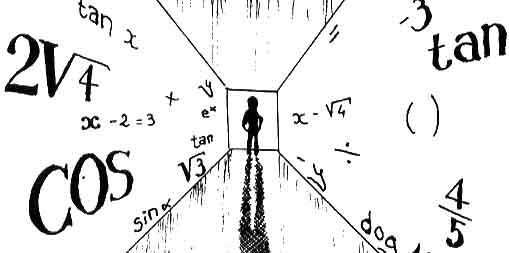
\includegraphics[scale=1]{math-theo}
\newpage


\newpage
\section{Matrices Théories}
\vspace{10mm} %5mm vertical space

\subsection{Les propriétés}
\vspace{5mm} %5mm vertical space

A) Linéarité \\

si on multiplie une matrice par $\lambda$, le déterminant est multiplié par $\lambda^{n}$ et toutes les lignes et colonnes sont multiplié par $\lambda=det(A)*\lambda^{n}$ \\
\vspace{5mm} %5mm vertical space

$
det(A+B) \neq det(A)+det(B) ? \\
$

Exemple:\\

$
A =
\begin{pmatrix}
  a & 0 \\
  0 & b \\
\end{pmatrix}
$
\vspace{5mm} %5mm vertical space
$
B =
\begin{pmatrix}
  c & 0 \\
  0 & d \\
\end{pmatrix}
$

\vspace{3mm} %5mm vertical space
det(A)=ab et det(B)=cd\\
\vspace{5mm} %5mm vertical space

Conclusion : \\

$
C =
\begin{pmatrix}
  a+c & 0 \\
  0 & b+d \\
\end{pmatrix}
$

\vspace{3mm} %5mm vertical space
$
det(C)=(a+c)*(b+d) \\
$

\vspace{3mm} %5mm vertical space
$\lambda^{n} \neq$ linéaire \\
$\lambda^{n}$ est exponentielle

\vspace{10mm} %5mm vertical space
B) Déterminant et transposée \\

Det(A) = det(A), les déterminants sont égaux, il y a juste la signature (le signe) qui est modifiée.\\

Démonstration :\\

$det(A) = \sum_{o \varepsilon s} \varepsilon (o^{-1}), ...$\\

$det(T_{a}) = \sum_{o \varepsilon s} \varepsilon (o^{1}), ...$

\vspace{10mm} %5mm vertical space
C) Déterminant et produit \\

les déterminants sont compatible avec le produit det(AB) = det(A) * det(B) \\

$
\varphi_{a} (x_{1}, ..., x_{n}) = det(\varphi_{c}) (A*1, ..., A*N))
$

\vspace{10mm} %5mm vertical space
D) Déterminant et matrice inversible \\

Une matrice est inversible uniquement si le déterminant est différents de 0. \\

$
det(A^{-1}) = \frac{1}{det(A)}
$

\subsection{Calcul du déterminants 2*2}
\vspace{5mm} %5mm vertical space
Le calcul du déterminants d'une matrice 2*2 est le résultat d'une soustraction entre la multiplications croisée des 2 ensembles \\
Il faut utiliser la ligne avec le plus de 0.

\vspace{5mm} %5mm vertical space

$
A =
\begin{pmatrix}
  1 & 4 \\
  2 & 3 \\
\end{pmatrix}
$

\vspace{5mm} %5mm vertical space

det(A) = (1*3) - (2*4)\\

det(A) = (3-8)\\

det(A) = (-5)\\

S = -5\\

\subsection{Calcul du déterminants 4*4 ou n*n}
\vspace{5mm} %5mm vertical space
Le calcul du déterminants d'une matrice n*n est le résultat d'une série d'opération entre les sous matrices.
\vspace{5mm} %5mm vertical space

$
A =
\begin{pmatrix}
  0 & 1 & 2 & 3 \\
  1 & 2 & 3 & 0 \\
  2 & 3 & 0 & 1 \\
  3 & 0 & 1 & 2 \\
\end{pmatrix}
$

\vspace{10mm} %5mm vertical space


$
A =
\begin{pmatrix}
  1 & 2 & 3 & 0 \\
  0 & 1 & 2 & 3 \\
  2 & 3 & 0 & 1 \\
  3 & 0 & 1 & 2 \\
\end{pmatrix}
$

\vspace{10mm} %5mm vertical space
Inversion de L1 avec L2\\

$
A =
\begin{pmatrix}
  \hl{\textbf{0}} & \hl{\textbf{1}} & \hl{\textbf{2}} & \hl{\textbf{3}} \\
  \hl{\textbf{1}} & \hl{\textbf{2}} & \hl{\textbf{3}} & \hl{\textbf{0}} \\
  2 & 3 & 0 & 1 \\
  3 & 0 & 1 & 2 \\
\end{pmatrix}
$
\vspace{5mm} %5mm vertical space

$
A =
\begin{pmatrix}
  \hl{\textbf{1}} & \hl{\textbf{2}} & \hl{\textbf{3}} & \hl{\textbf{0}} \\
  \hl{\textbf{0}} & \hl{\textbf{-1}} & \hl{\textbf{-2}} & \hl{\textbf{-3}} \\
  2 & 3 & 0 & 1 \\
  3 & 0 & 1 & 2 \\
\end{pmatrix}
$

\vspace{10mm} %5mm vertical space
Méthodes du pivot de Gauss \\

\vspace{10mm} %5mm vertical space
Mise à zero de L3 \\
L3 - (2*L1) = L3 \\

$
A =
\begin{pmatrix}
  1 & 2 & 3 & 0 \\
  0 & -1 & -2 & -3 \\
  \hl{\textbf{2-(1*2)}} & \hl{\textbf{3-(2*2)}} & \hl{\textbf{0-(2*3)}} & \hl{\textbf{1-(2*0)}} \\
  3 & 0 & 1 & 2 \\
\end{pmatrix}
$

\vspace{5mm} %5mm vertical space

$
A =
\begin{pmatrix}
  1 & 2 & 3 & 0 \\
  0 & -1 & -2 & -3 \\
  \hl{\textbf{(2-2)}} & \hl{\textbf{3-4}} & \hl{\textbf{(0-6)}} & \hl{\textbf{1-0)}} \\
  3 & 0 & 1 & 2 \\
\end{pmatrix}
$

\vspace{5mm} %5mm vertical space

$
A =
\begin{pmatrix}
  \hl{\textbf{1}} & 2 & 3 & 0 \\
  0 & -1 & -2 & -3 \\
  0 & -1 & -6 & 1 \\
  3 & 0 & 1 & 2 \\
\end{pmatrix}
$

\vspace{10mm} %5mm vertical space

Mise à zero de L4 \\
L4 - (3*L1) = L4 \\

$
A =
\begin{pmatrix}
  \hl{\textbf{1}} & 2 & 3 & 0 \\
  0 & -1 & -2 & -3 \\
  0 & -1 & -6 & 1 \\
  \hl{\textbf{3-(3*1)}} & \hl{\textbf{0-(3*2)}} & \hl{\textbf{1-(3*3)}} & \hl{\textbf{2-(3*0)}} \\
\end{pmatrix}
$

\vspace{5mm} %5mm vertical space

$
A =
\begin{pmatrix}
  \hl{\textbf{1}} & 2 & 3 & 0 \\
  0 & -1 & -2 & -3 \\
  0 & -1 & -6 & 1 \\
  \hl{\textbf{3-3}} & \hl{\textbf{0-6}} & \hl{\textbf{1-9}} & \hl{\textbf{2-0}} \\
\end{pmatrix}
$

\vspace{5mm} %5mm vertical space

$
A =
\begin{pmatrix}
  1 & 2 & 3 & 0   \\
  0 & -1 & -2 & -3   \\
  0 & -1 & -6 & 1 \\
  0 & -6 & -8 & 2 \\
\end{pmatrix}
$

A partir de ce moment-ci, nous pouvons utiliser la formule de sarus, liebniz, ... \\
Exmples: \\

\subsection{Méthode Elimination de Gauss} \\

\vspace{5mm} %5mm vertical space

$
A =
\begin{pmatrix}
  1 & 2 & 3 & 0   \\
  0 & \hl{\textbf{-1}} & -2 & -3   \\
  0 & -1 & -6 & 1 \\
  0 & -6 & -8 & 2 \\
\end{pmatrix}
$

\vspace{5mm} %5mm vertical space

L3 = L3-1*L2 \\

$
A =
\begin{pmatrix}
  1 & 2 & 3 & 0    \\
  0 & \hl{\textbf{-1}} & -2 & -3 \\
  0 & \hl{\textbf{0}} & \hl{\textbf{-4}} & \hl{\textbf{4}}   \\
  0 & -6 & -8 & 2  \\
\end{pmatrix}
$

\vspace{5mm} %5mm vertical space

L4 = L4-6*L2 \\

\vspace{5mm} %5mm vertical space

$
A =
\begin{pmatrix}
  1 & 2 & 3 & 0    \\
  0 & \hl{\textbf{-1}} & -2 & -3 \\
  0 & 0 & -4 & 4   \\
  0 & \hl{\textbf{0}} & \hl{\textbf{4}} & \hl{\textbf{20}}   \\
\end{pmatrix}
$

\vspace{5mm} %5mm vertical space

$
A =
\begin{pmatrix}
  1 & 2 & 3 & 0    \\
  0 & -1 & -2 & -3 \\
  0 & 0 & \hl{\textbf{-4}} & 4   \\
  0 & 0 & 4 & 20  \\
\end{pmatrix}
$

\vspace{5mm} %5mm vertical space

L4-(-1)*L3\\

\vspace{5mm} %5mm vertical space

$
A =
\begin{pmatrix}
  1 & 2 & 3 & 0    \\
  0 & -1 & -2 & -3 \\
  0 & 0 & \hl{\textbf{-4}} & 4   \\
  \hl{\textbf{0}} & \hl{\textbf{0}} & \hl{\textbf{0}} & \hl{\textbf{24}}  \\
\end{pmatrix}
$

\vspace{5mm} %5mm vertical space
Fin de la triangulaire Suppérieures \\

$
A =
\begin{pmatrix}
  1 & 2 & 3 & 0    \\
  \hl{\textbf{0}} & -1 & -2 & -3 \\
  \hl{\textbf{0}} & \hl{\textbf{0}} & -4 & 4   \\
  \hl{\textbf{0}} & \hl{\textbf{0}} & \hl{\textbf{0}} & 24  \\
\end{pmatrix}
$

\vspace{5mm} %5mm vertical space

1*(-1)*(-4)*24=\hl{\textbf{96}} \\
\vspace{4mm} %5mm vertical space
S= det(A) = \hl{\textbf{96}} \\

\subsection{Autres Méthode} \\

Elimination en matrice 3*3 \\

\vspace{5mm} %5mm vertical space

$
A =
\begin{pmatrix}
  \hl{\textbf{1}} & 2 & 3 & 0   \\
  \hl{\textbf{0}} & -1 & -2 & -3   \\
  \hl{\textbf{0}} & -1 & -6 & 1 \\
  \hl{\textbf{0}} & -6 & -8 & 2 \\
\end{pmatrix}
$

\vspace{5mm} %5mm vertical space

$
A = 1*( \\
  \begin{pmatrix}
     2 & 3 & 0   \\
    -1 & -2 & -3 \\
    -1 & -6 & 1  \\
    -6 & -8 & 2  \\
  \end{pmatrix}
)\\
$

\vspace{5mm} %5mm vertical space

Création de la matrice de signe \\

$
A = 1*( \\
  \begin{pmatrix}
    + & - & +  \\
    - & + & -  \\
    + & - & +  \\
    - & + & -  \\
  \end{pmatrix}
)\\
$


\vspace{5mm} %5mm vertical space

Création de la matrice de signe \\

$
A =
1*( \\
  1*( \\
  \begin{pmatrix}
    6 & 1 \\
    8 & 2 \\
  \end{pmatrix}
  ) \\
  -2*( \\
  \begin{pmatrix}
    1 & 1 \\
    6 & 2 \\
  \end{pmatrix}
  ) \\
  3*( \\
  \begin{pmatrix}
    1 & 6 \\
    6 & 8 \\
  \end{pmatrix}
  )\\
)\\
$

\vspace{5mm} %5mm vertical space

Création de la matrice de signe \\

$
A =
1*( \\
  1*( (6*2)-(8*1) )  \\
  -2*( (1*2)-(6*1) ) \\
  3*( (1*8)-(6*6) )  \\
) \\
$

\vspace{5mm} %5mm vertical space

$
A =
1*( \\
  1*( (12)-(8) )  \\
  -2*( (2)-(6) ) \\
  3*( (8)-(36) )  \\
) \\
$

\vspace{5mm} %5mm vertical space

$
A =
1*( \\
  (1*4)  \\
  - (2*(-4)) \\
  - (3*(-28))  \\
) \\
$

\vspace{5mm} %5mm vertical space
4−(−8)−(−84)=\hl{\textbf{96}} \\

\vspace{4mm} %5mm vertical space
S= det(A) = \hl{\textbf{96}} \\

\newpage
\chapter{Nombres Complexes}
\vspace{3mm} %5mm vertical space
\section{Conversion polaire - cartésienne}
\vspace{3mm} %5mm vertical space

\textbf{Définition du module} \\

le module noté $|Z|$ est la longueur du segment (rayon). Elle peut être mesurée  grâce à la formule de pythagore ($\sqrt{a²+b²}$). \\


\vspace{5mm} %5mm vertical space
\textbf{Représentation Géographique} \\

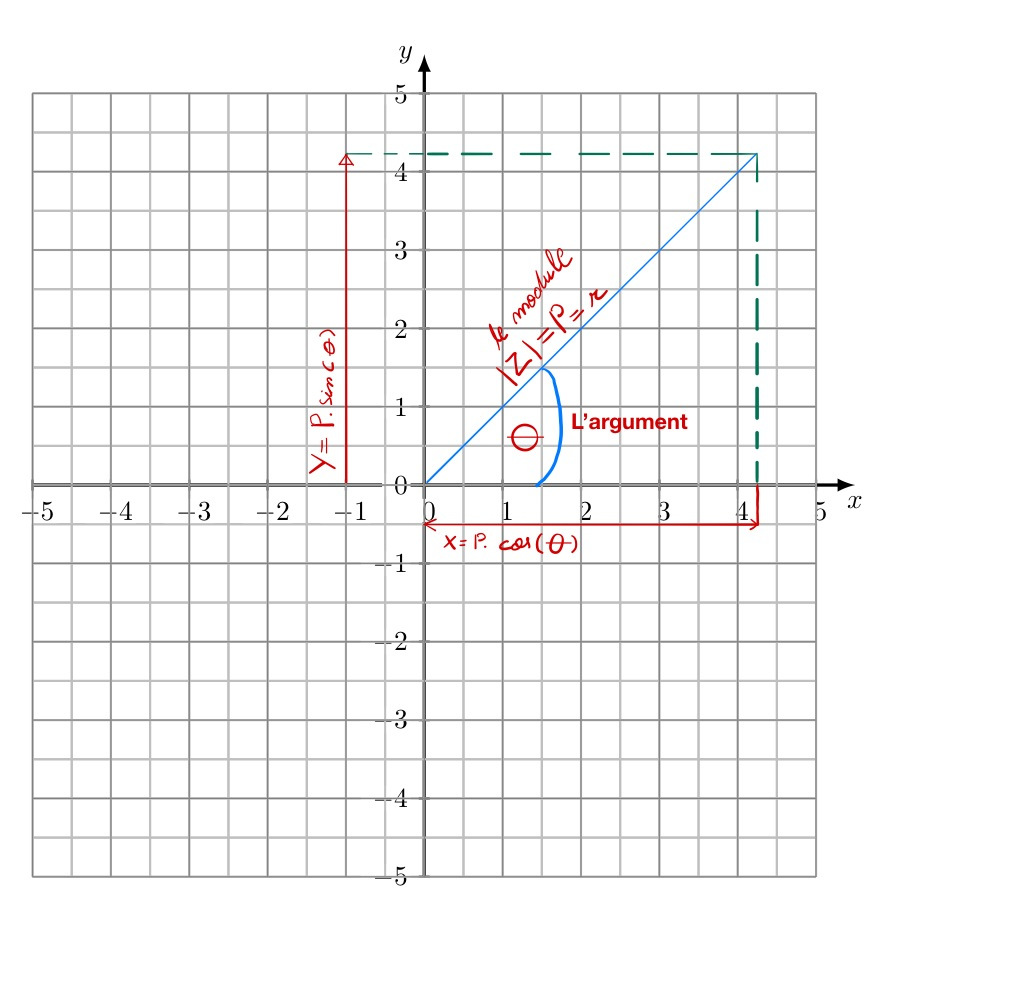
\includegraphics[scale=1.5]{cart-mod}

\textbf{Démonstration}\\

$|Z| = \rho cos(\theta)+ \rho sin(\theta) *i$ \\
$|Z| = \sqrt(\rho^{2} cos(\theta)^{2}+ \rho^{2} sin(\theta)^{2})$ \\
$|Z| = \sqrt(\rho^{2} cos(\theta)^{2}+ sin(\theta))*i $ \\
$|Z| = \sqrt(\rho^{2}) $ \\
$|Z| = \rho $ \\

$\rho$ est le module et $\theta$ est l'argument \\
$Z = P(cos(\theta) + sin(\theta)*i )$ ou $Z= P(cis(\theta))$\\

\newpage

\section{Conversion Cartésienne - Polaire}
\vspace{3mm} %5mm vertical space

$\rho$ = $\sqrt{x²+y²}$ \\

\textbf{Démonstration Géométriquement} \\

Nous pouvons voir que $\theta$ est modifié en fonction de X et de Y que si nous dessinons un cercle, nous pouvons voir que le segment Y est une tangeante au cercle de rayon X. \\

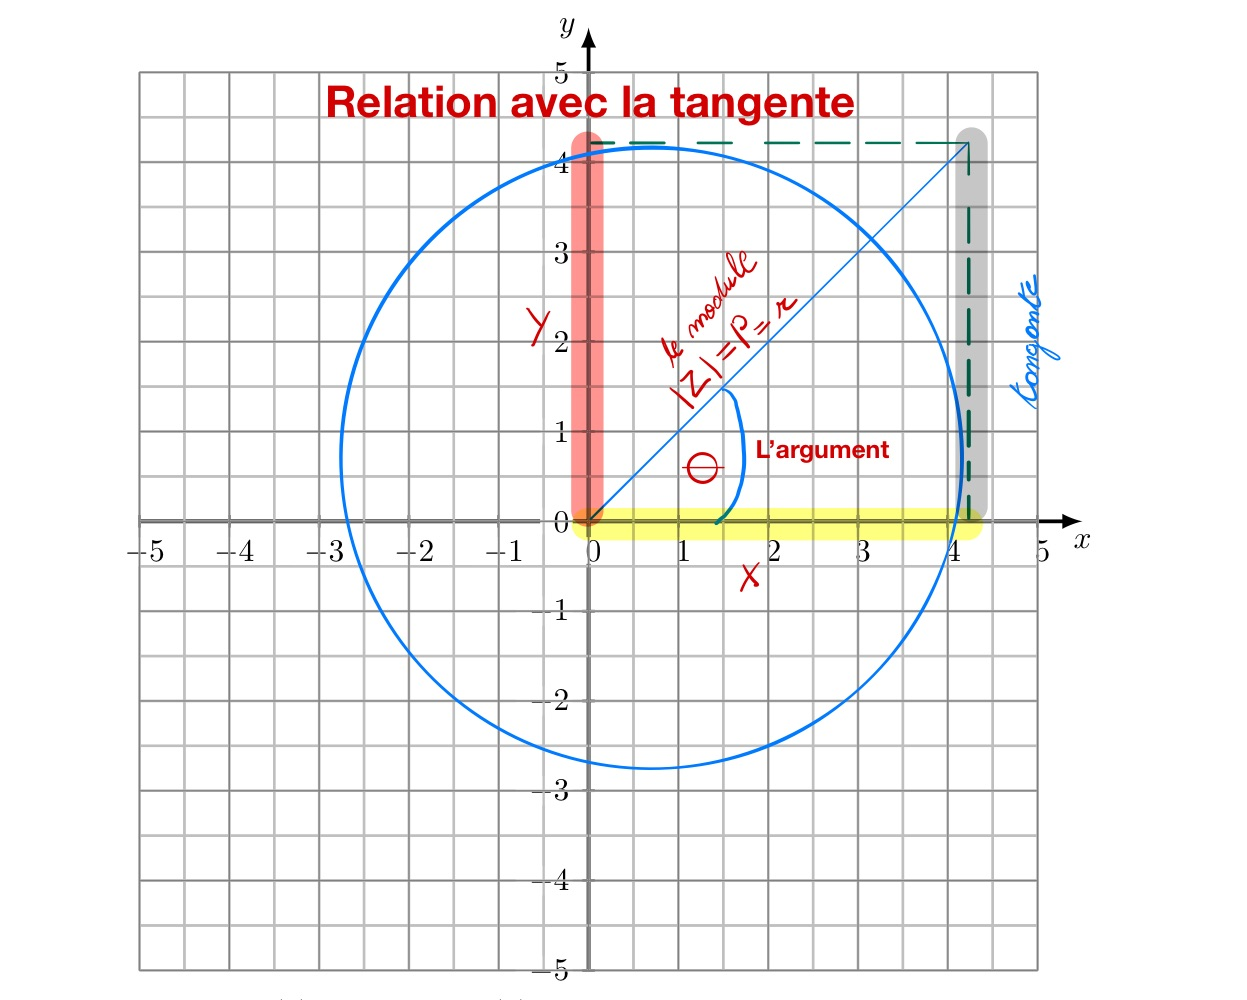
\includegraphics[scale=0.3]{cart-tg}

$X=\rho * cos(\theta)$ $ $ $ Y=\rho * sin(\theta)$

\vspace{5mm} %5mm vertical space
\textbf{Démonstration Algébriquement} \\

$\frac{Y}{X}$ = $\frac{\rho * sin(\theta)}{\rho * cos(\theta)}$ \\
$\frac{Y}{X}$ = $\frac{sin(\theta)}{cos(\theta)}$ \\
$\frac{Y}{X}$ = tg($\theta)$ \\

\vspace{5mm} %5mm vertical space
\textbf{Conclusion} \\

$\theta = arctg(\frac{Y}{X})$ \\
$tg(\theta) = \frac{Y}{X}$ \\


\newpage

\section{Conversion cartésienne/polaire - exponentielle}
\vspace{3mm} %5mm vertical space

tout nombre complexes peut s'écrire sous la formes : $\rho * e^{i\theta}$ \\

\textbf{Ecriture cartésienne} \\

$1+\sqrt{3}i$ = x + yi \\

\vspace{5mm}
\textbf{Etape 1: Trouver $\rho$ (calcul du module)} \\

$\rho = \sqrt{x^{2} + y^{2}}$ \\

$\rho = \sqrt{1^{2} + \sqrt{3}^{2}}$ \\

$\rho = \sqrt{1 + 3}$ \\

$\rho = \sqrt{4 => 2^{2}}$ \\

$\rho = 2$ \\

\vspace{5mm}
\textbf{Etape 2: Trouver $\theta$ (calcul de l'argument)} \\

$\theta = artg(\frac{y}{x})$ \\

$\theta = arctg(\frac{1}{\sqrt{3}})$ \\

$tg(\theta) = \frac{1}{\sqrt{3}} * \frac{\sqrt{3}}{\sqrt{3}}$ \\

$tg(\theta) = \frac{1\sqrt{3}}{\sqrt{3}^{2}}$ \\

$tg(\theta) = \frac{\sqrt{3}}{3})$ ou $artg(\frac{\pi}{6}) $ \\

$tg(\theta) = \frac{\pi}{6} $ \\


\vspace{5mm}
\textbf{Etape 3: Ecriture sous le format exponentielle} \\

$2e^{\frac{\pi}{6}i}$


\newpage
\section{Conversion exponentielle - polaire/cartésienne }
\vspace{3mm} %5mm vertical space

\textbf{Ecriture exponentielle} \\

$e^{1+\frac{\pi}{2}i}$ \\

\textbf{Simplification} \\

$e^{1+\frac{\pi}{2}i}$ \\

$e^{1} + e^{\frac{\pi}{2}i}$ \\

$e*cis(\frac{\pi}{2})$ \\

$e*(cos(\frac{\pi}{2}) + i*sin(\frac{\pi}{2})) $ \\

$e*(cos(\frac{\pi}{2}) + i*sin(\frac{\pi}{2})) $ \\

$e*(0 + i*1) $ \\

$e*i $ \\


\newpage
\section{Nombre Complexes addition}
\vspace{3mm} %5mm vertical space

$(4 * cis(45^{\circ} )) + (5 * cis(\frac{\pi}{3}))$

\vspace{10mm}
\textbf{Calcul du module}
\vspace{5mm}

$\rho = \sqrt{\rho_{1}^{2} + \rho_{2}^{2} + \rho_{1} \rho_{2} cos(\theta_{1} - \theta_{2}) }$ \\

$\rho = \sqrt{4^{2} + 5^{2} + 2 * 4 * 5 cos(45^{\circ} - 60^{\circ})}$ \\

$\rho = \sqrt{41 + 40 * 0,96592582628}$ \\

$\rho = \sqrt{79,6370330512}$ \\

$\rho = 8,923958373457376 $ \\

\vspace{6mm}
\textbf{Calcul de l'argument}
\vspace{5mm}

$\theta = arctg(\frac{\rho_{1}sin(\theta_{1}) + \rho_{2}sin(\theta_{2})} {\rho_{1}cos(\theta_{1}) + \rho_{2}cos(\theta_{2})} )$ \\

$\theta = arctg(\frac{4sin(45^{\circ}) + 5sin(60^{\circ})} {4cos(45^{\circ}) + 5cos(60^{\circ})} )$ \\

$\theta = arctg(\frac{4\frac{\sqrt{2}}{2}) + 5\frac{\sqrt{3}}{2} } {4\frac{\sqrt{2}}{2}) + 5\frac{1}{2}})$ \\

$\theta = arctg(1.3434647741399612)$ \\

$\theta = arctg(53.3380661^{\circ})$ \\

\vspace{6mm}
\textbf{Solution}
\vspace{5mm}

$|Z| = 8,923 cis(53.338^{\circ})$


\newpage
\section{Nombre Complexes soustraction}
\vspace{3mm} %5mm vertical space

$(4 * cis(45^{\circ} )) - (5 * cis(\frac{\pi}{3}))$


\vspace{6mm}
\textbf{Calcul du modules}
\vspace{5mm}

$\rho = \sqrt{\rho_{1}^{2} + \rho_{2}^{2} + 2*\rho_{1}*\rho_{2} cos(\theta_{1} -  \theta_{2})}$ \\

$\rho = \sqrt{4^{2} + 5^{2} +2*4*5* cos(45^{\circ} - \frac{\pi}{3})}$ \\

$\rho = \sqrt{4^{2} + 5^{2} + 40* cos(45^{\circ} - 60^{\circ})}$ \\

$\rho = \sqrt{16 + 25 + 40* 0,965925826}$ \\

$\rho = \sqrt{79,637033052}$ \\

$\rho = 8,923958374$ \\

\vspace{4mm}
\textbf{Calcul de l'argument}
\vspace{5mm}

$\theta = arctg(\frac{\rho_{1}*sin(\theta_{1}) - \rho_{2}*sin(\theta_{2})}{\rho_{1}*cos(\theta_{1}) - \rho_{2}*cos(\theta_{2})})$ \\

$\theta = arctg(\frac{4*sin(45^{\circ}) - 5*sin(\frac{\pi}{3})}{4*cos(45^{\circ}) - 5*cos(\frac{\pi}{3})})$ \\

$tg(\theta) = \frac{4*sin(45^{\circ}) - 5*sin(60^{\circ})}{4*cos(45^{\circ}) - 5*cos(60^{\circ})}$ \\

$tg(\theta) = \frac{4\frac{\sqrt{2}}{2} - 5\frac{\sqrt{3}}{2} } {4*\frac{1}{2} - 5 * \frac{\sqrt{2}}{2}}$ \\

$tg(\theta) = \frac{2\sqrt{2} - \frac{5\sqrt{3}}{2} } {2 - \frac{5\sqrt{2}}{2} }$ \\

$tg(\theta) = \frac{\frac{4\sqrt{2} - 5\sqrt{3}}{2}} {\frac{4 - 5\sqrt{3}}{2} }$ \\

$tg(\theta) = \frac{4\sqrt{2} - 5\sqrt{3}} {4 - 5\sqrt{3} }$ \\

$tg(\theta) = - \frac{(4\sqrt{2} - 5\sqrt{3}) * (4\sqrt{2} - 5\sqrt{3})}{59}$ \\

$tg(\theta) = - \frac{(16\sqrt{2} + 20\sqrt{6} - 20\sqrt{3} - 75)} {59}$ \\

$tg(\theta) = 0,644471$ \\

$tg(\theta) = 36,93^{\circ}$ \\


\vspace{6mm}
\textbf{Solution}
\vspace{5mm}

$|Z| = 8,923958374*cis(36,93^{\circ})$ \\

\newpage
\section{Nombre Complexes multiplication}
\vspace{3mm} %5mm vertical space

$(4 * cis(45^{\circ} )) * (5 * cis(\frac{\pi}{3}))$ \\

$|Z| = \rho_{1}\rho_{2}( cos(\theta_{1} + \theta_{2}) + i*(sin(\theta_{1} + \theta_{2})) )$ \\

$|Z| = (\rho_{1}\rho_{2})*cis(\theta_{1} + \theta_{2})$ \\


\vspace{6mm}
\textbf{Calcul du modules}
\vspace{5mm}

$\rho = \rho_{1}\rho_{2}$ \\

$\rho = 4*5 $ \\

$\rho = 20 $ \\

\vspace{6mm}
\textbf{Calcul de l'argument}
\vspace{5mm}

$\theta = \theta_{1}+\theta_{2}$ \\

$\theta = 45^{\circ} + \frac{\pi}{3}$ \\

$\theta = 45^{\circ} + 60^{\circ}$ \\

$\theta = 105^{\circ}$ \\

\vspace{6mm}
\textbf{Solution}
\vspace{5mm}

$|Z| = 20 * cis(105^{\circ})$

\newpage
\section{Nombre Complexes division}
\vspace{3mm} %5mm vertical space

$\frac{(4 * cis(45^{\circ} ))} {(5 * cis(\frac{\pi}{3}))} $ \\

$|Z| = (\frac{\rho_{1}}{\rho_{2}})* cis(\theta_{1} - \theta_{2})$ \\

\vspace{6mm}
\textbf{Calcul du modules}
\vspace{5mm}

$\rho = \frac{4}{5}$ \\

\vspace{6mm}
\textbf{Calcul de l'argument}
\vspace{5mm}

$\theta = 45^{\circ} - \frac{\pi}{3} $ \\

$\theta = 45^{\circ} - 60^{\circ} $ \\

$\theta = - 15^{\circ} $ \\

\vspace{6mm}
\textbf{Solution}
\vspace{5mm}

$ |Z| = \frac{4}{5} * cis(- 15^{\circ})$ \\

\newpage

\section{Chaptire 3 : Logique}
\vspace{5mm} %5mm vertical space

\subsection{Logique propositionnelle}
\vspace{5mm} %5mm vertical space

Règles pour déterminer si c'est vrai ou faux: \\

1) Principe d'identité : A=A \\

2) Non contradiction : On ne peut pas nier et affirmer la même chose ¬A et A \\

3) Tiers Exlus : Quelques chose existe ou dois ne pas exister A ou ¬A \\


\subsection{Proposition}
\vspace{5mm} %5mm vertical space

C'est un énoncé, une phrase simple : \\
ex: Ceci est une vidéos $=>$ Vrai ou Faux \\

En logique propositionnelle les propositions ne peuvent qu'être vrai ou fausse \\

exemple de proposition : \\
2+2 $=>$ Vrai ou Faux \\
Le mur est blanc $=>$ Vrai ou Faux \\

\subsection{L'implication}
\vspace{5mm} %5mm vertical space

Si j'ai une proposition A alors B \\

Exemple: \\
Une paire de chaussure $=>$ j'ai 2 chaussures \\
Une paire de chaussure implique que j'ai 2 chaussures \\
A$=>$B : Faux (une paire nécessite d'avoir 2 même chaussures, 2 chaussures peuvent être différentes)\\
Si A est vrai alors B est vrai \\
si B est vrai alors A n'est pas forcément vrai \\

\subsection{L'équivalence}
\vspace{5mm} %5mm vertical space

Il faut que je n'ai pas une paires de chaussures. \\
A=B : vrai \\
Si A est vrai alors B est vrai \\
si B est vrai alors A est vrai \\

\subsection{Vocabulaire}
\vspace{5mm} %5mm vertical space

Proposition Atomique : Vrai et Faux à la fois \\
Tautologie : toujours vrai \\
prédicats :  Pour tout il existe \\



\subsection{Tableau priorités logique}
\begin{tabular}{|l|c|c|c|c|}
  \hline
  Opérateur & Logic & priorités & Associativités .\\
  \hline
  $<=>$ & Equalité & 1 & gauche \\
  $=>$ & Implications & 2 & droite \\
  V & OU & 3 & gauche \\
  ∧ & ET & 4 & gauche \\
  ¬ & NON & 5 & gauche \\
  \hline
\end{tabular}


\subsection{Tautologie}
\begin{tabular}{|l|c|c|c|}
  \hline
  P & ¬ P & P V ¬P \\
  \hline
  T & T & ⊥ \\
  ⊥ & T & T \\
  \hline
\end{tabular}

\subsection{Changement de forme}
\vspace{5mm} %5mm vertical space
Commutativité: \\
pvq = qvp \\
p∧q = q∧p \\

\vspace{5mm} %5mm vertical space
Associativités: \\
(pvq)vr = pv(qvr) \\
(p∧q)∧r = p∧(q∧r) \\

\vspace{5mm} %5mm vertical space
Distributivités: \\
pv(q∧r) = (pvq)∧(pvr) \\
pv(qvr) = (p∧q)v(p∧r) \\

\vspace{5mm} %5mm vertical space
De Morgans: \\
a v b= ¬a * ¬b\\
a*b= ¬a + ¬b\\
(p∧q) = ¬p v ¬q  \\
(pvq) = ¬ (¬p ∧ ¬q)  \\
¬(p∧q) = (p v q)  \\
(A ∧¬ B) V (¬ A V (C ∧ A)) =  ¬(A ∧¬ B) ∧ ¬(¬ A V (C ∧ A))\\

\vspace{5mm} %5mm vertical space
Forme conjonctive: \\
(A ET B) OU C \\
(A ∧ B) V C\\

\vspace{5mm} %5mm vertical space
Forme disjonctive : \\
(A OU B) ET C \\
(A V B) ∧ C\\

\vspace{5mm} %5mm vertical space
Transformation: \\
A$=>$B = ¬A v (A∧B) \\
A$<=>$B: = (A$=>$B)∧(B$=>$A)  \\
(A$=>$B)∧(B$=>$A) = (¬A v (A∧B)) ∧ (¬B v (B∧A))

\newpage

\chapter{Théorie naïve des ensembles}
\vspace{4mm} %5mm vertical space

\section{Définition}

on appelle ensemble, une collection d'objets appellés éléments de cet ensemble.\\
un objet particulier appartient ($\in$) ou n'appartient pas ($\notin$) à un ensemble donné.\\

Exemple d'ensemble : l'ensemble des voyelles : V=\{a,e,i,o,u,y\} \\

a $\in$ V : a appartient à l'ensemble V \\
d $\notin$ V : d n'appartient pas à l'ensemble V \\

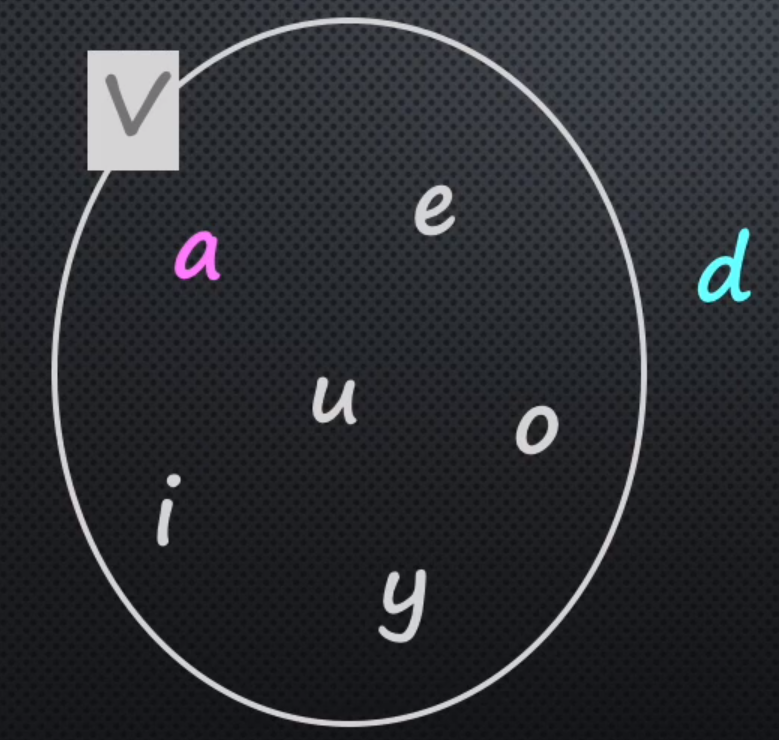
\includegraphics[scale=0.2]{Ensembles}
\vspace{3mm} %5mm vertical space

\section{Relation d'inclusion}

Soient A et B sont deux ensembles, on dit que A est inclus dans B (Noté A$\subset$ B), si tout les éléments de A sont des éléments de B.
Autrement dit (X$\subset$A) et que (X$\subset$B).\\

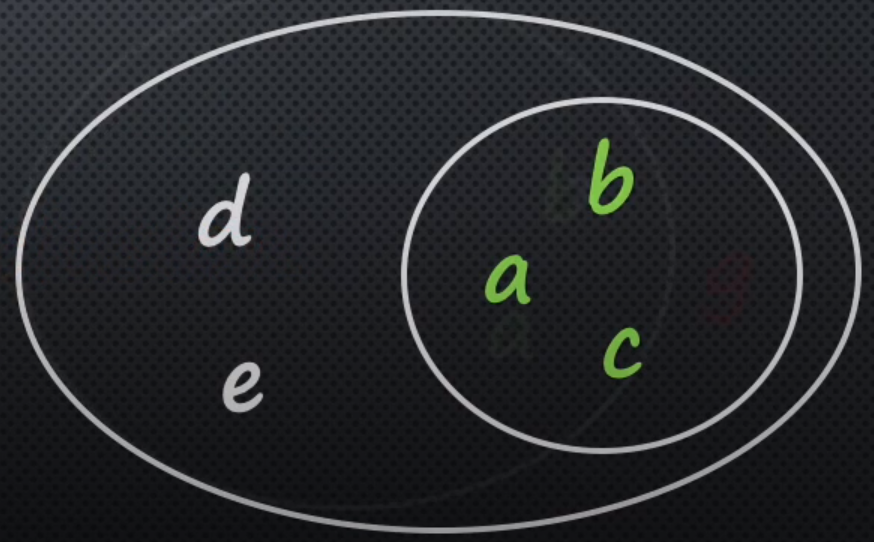
\includegraphics[scale=0.2]{EnsemblesInc}
\vspace{3mm} %5mm vertical space

On peut dire que \{a,b,g\}$\in$\{a,b,d,e\} \\

\section{Propriété de l'inclusion}

\begin{itemize}
\item {a. Reflexivité : pour tout ensemble A (A$\in$B)}
\item {b. Anti-Symétrique : (A$\in$B) et (B$\in$A) $=>$ A=B}
\item {c. Transitivité : (A$\in$B) et (B$\in$C) $=>$ (A$\in$C)}
\end{itemize}

\newpage
\section{Relation d'égalité}

Soient A et B sont deux ensembles, on dit que A égale B (Noté A=B), si tout les éléments de A appartient à B. Autrement dit (X$\in$A) et que (X$\in$B).

\section{Opération d'union ($\cup$)}
\vspace{3mm} %5mm vertical space

1) L'union de 2 ensembles \\

A= \{a,e\} et B = \{b,c,d\} \\

C = A $\cup$ B = \{a,e,b,c,d\}

\vspace{3mm} %5mm vertical space
\section{Opération d'intersection ($\cap$)}
\vspace{3mm} %5mm vertical space

\textbf{Intersection de 2 ensembles} \\

Soient A et B deux ensembles, on appelle (A$\cap$B) le nouvel ensemble contenant les éléments se trouvant dans A et B. \\

A= \{a,b\} et B = \{b,c,d\} \\

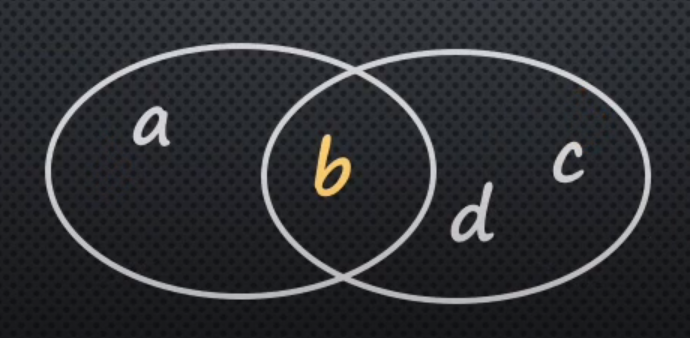
\includegraphics[scale=0.2]{EnsemblesInt}
\vspace{3mm} %5mm vertical space

C = A $\cap$ B = \{b\} \\

\section{Ensemble vide}

L'ensemble vide est une partie (un sous-ensemble) de n'importe quel ensembles.\\
Il ne possède qu'un seul sous-ensemble : lui-même \\

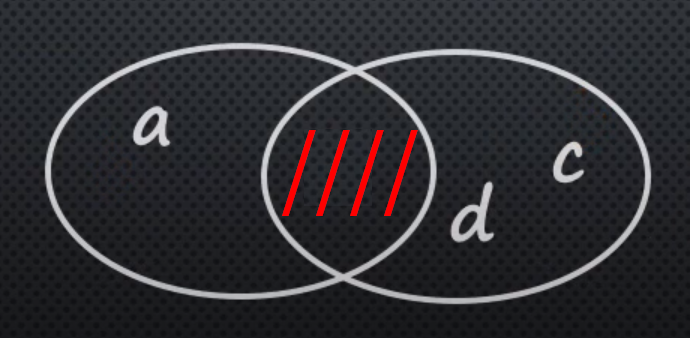
\includegraphics[scale=0.2]{EnsemblesVide}
\vspace{3mm} %5mm vertical space

C = A $\cap$ B = \{$\oslash$\}

\newpage
\section{Cardinalité}

Soit A un ensemble, Si A possède exactement N éléments (n $\in$ \N), A est un ensemble fini de cardinalité N.\\

Noté $|A|$ = n \\

$|1,2,3|$ = 3 \\

$|\oslash|$ = 0 \\

$|\{\oslash\}|$ = 1 \\

\section{Identité}

A $\cup$ A = A \\
A $\cap$ A = A \\

\section{Commutativité}

A $\cap$ B  = B $\cap$ A \\
A $\cup$ B  = B $\cup$ A \\

\section{Associativité}

A $\cap$ (B $\cap$ C) = (A $\cap$ B) $\cap$ C \\
A $\cup$ (B $\cup$ C) = (A $\cup$ B) $\cup$ C \\

\section{Distributivité}

A $\cap$ (B $\cup$ C) = (A $\cap$ B) $\cup$ (A $\cap$ C) \\
A $\cup$ (B $\cap$ C) = (A $\cup$ B) $\cap$ (A $\cup$ C) \\

\section{De Morgans}

¬(A $\cup$ B) = ¬A $\cap$ ¬B) \\
¬(A $\cap$ B) = ¬A $\cup$ ¬B) \\



\newpage

\vspace{30mm}
\textbf{\Huge{Mathématiques Exercices}}

\vspace{50mm}
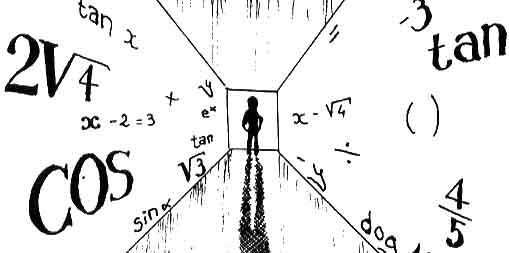
\includegraphics[scale=1]{math-theo}
\newpage


\newpage
\section{Exercice Matrices}
\vspace{10mm} %5mm vertical space
\subsection{Enoncés des exercices}
\vspace{5mm} %5mm vertical space

$
A =
\begin{pmatrix}
  0 & 1 & 2 & 3 \\
  1 & 2 & 3 & 0 \\
  2 & 3 & 0 & 1 \\
  3 & 0 & 1 & 2 \\
\end{pmatrix}
$
\vspace{5mm} %5mm vertical space
$
B =
\begin{pmatrix}
  1 & 4 \\
  2 & 3 \\
  3 & 2 \\
  4 & 1 \\
\end{pmatrix}
$
\vspace{5mm} %5mm vertical space
$
C =
\begin{pmatrix}
  1 & 2 & 3 & 4 \\
  4 & 3 & 2 & 1 \\
\end{pmatrix}
$
\vspace{3mm} %5mm vertical space

\begin{enumerate}[label=\Alph*)]
\item Calculer B*C
\item Calculer la trace de A
\item Calculer la transposée de B
\item Calculer 2,5*C
\item Calculer $B^{t}+C$
\item Calculer le déterminants de A
\item Exercices d'examens
\item Exercices supplémentaire (Déplacement 3D)
\end{enumerate}

\newpage

\subsection{Résolution des exercices}
\vspace{5mm} %5mm vertical space
A) Calculer B*C
\vspace{10mm} %5mm vertical space

$
B*C =
\begin{pmatrix}
  1*1+4*4 & 1*2+4*3 & 1*3+4*2 & 1*4+4*1 \\
  2*1+3*4 & 2*2+3*3 & 2*3+3*2 & 2*4+3*1 \\
  3*1+2*4 & 3*2+2*3 & 3*3+2*2 & 3*4+2*1 \\
  4*1+1*4 & 4*2+1*3 & 4*3+1*2 & 4*4+1*1 \\
\end{pmatrix}
$

\vspace{5mm} %5mm vertical space

$
S = B*C =
\begin{pmatrix}
  17 & 14 & 11 & 8 \\
  14 & 13 & 12 & 10 \\
  11 & 12 & 13 & 15 \\
  8 & 11 & 14 & 17 \\
\end{pmatrix}
$

\vspace{10mm} %5mm vertical space
B) Calculer la trace de A
\vspace{5mm} %5mm vertical space

La trace d'une matrices est la somme de chaque éléments de sa diagonale
\vspace{5mm} %5mm vertical space

$
A =
\begin{pmatrix}
  \hl{\textbf{0}}  & 1 & 2 & 3 \\
  1 & \hl{\textbf{2}} & 3 & 0 \\
  2 & 3 & \hl{\textbf{0}} & 1 \\
  3 & 0 & 1 & \hl{\textbf{2}} \\
\end{pmatrix}
$
\vspace{3mm} %5mm vertical space

La trace de la matrice A = 0+2+0+2 = 4 \\
S = 4 \\

\vspace{10mm} %5mm vertical space
C) Calculer la transposée de la matrice B

\vspace{4mm} %5mm vertical space
La transposée de la matrice est d'intervertir les lignes/colonnes de la matrice originale.

\vspace{5mm} %5mm vertical space
$
B =
\begin{pmatrix}
  1 & 4 \\
  2 & 3 \\
  3 & 2 \\
  4 & 1 \\
\end{pmatrix}
$
\vspace{5mm} %5mm vertical space
$
B^{t} =
\begin{pmatrix}
  1 & 2 & 3 & 4 \\
  4 & 3 & 2 & 1 \\
\end{pmatrix}
$

Notes : $B^{t}$ est égale à C \\

$
B^{t} = C =
\begin{pmatrix}
  1 & 2 & 3 & 4 \\
  4 & 3 & 2 & 1 \\
\end{pmatrix}
$

\vspace{5mm} %5mm vertical space

S = $B^{t}$ ou C\\

\vspace{10mm} %5mm vertical space
D) Calculer 2,5*C

\vspace{5mm} %5mm vertical space
$
2,5*C =
\begin{pmatrix}
  1*2,5 & 2*2,5 & 3*2,5 & 4*2,5 \\
  4*2,5 & 3*2,5 & 2*2,5 & 1*2,5 \\
\end{pmatrix}
$
\vspace{5mm} %5mm vertical space

$
S = 2,5*C =
\begin{pmatrix}
  2,5 & 5 & 7,5 & 10 \\
  10 & 7,5 & 5 & 2,5 \\
\end{pmatrix}
$


\vspace{10mm} %5mm vertical space
E) Calculer $B^{t} + C$

\vspace{5mm} %5mm vertical space
$
B^{t} = C =
\begin{pmatrix}
  1 & 2 & 3 & 4 \\
  4 & 3 & 2 & 1 \\
\end{pmatrix}
$
\vspace{5mm} %5mm vertical space

Notes : $B^{t} = C$ = C+C ou 2*C
\vspace{5mm} %5mm vertical space

$
S = 2*C =
\begin{pmatrix}
  1*2 & 2*2 & 3*2 & 4*2 \\
  4*2 & 3*2 & 2*2 & 1*2 \\
\end{pmatrix}
$

\vspace{5mm} %5mm vertical space
S = $ B^{t}$ +C = 2*C = C+C = \\

$
\begin{pmatrix}
  2 & 4 & 6 & 8 \\
  8 & 6 & 4 & 2 \\
\end{pmatrix}
$

\vspace{10mm} %5mm vertical space

F) Calcul du déterminant \\

$
A =
\begin{pmatrix}
  0 & 1 & 2 & 3 \\
  1 & 2 & 3 & 0 \\
  2 & 3 & 0 & 1 \\
  3 & 0 & 1 & 2 \\
\end{pmatrix}
$

\vspace{10mm} %5mm vertical space

Extraction des sous matrices \\

\vspace{5mm} %5mm vertical space
Matrices de signes \\

\vspace{5mm} %5mm vertical space

$
\begin{pmatrix}
  + & + & - & + \\
  - & - & + & - \\
  + & + & - & + \\
  - & + & + & - \\
\end{pmatrix}
$

\vspace{10mm} %5mm vertical space
Extraction des matrices \\
\vspace{5mm} %5mm vertical space

$
-1*(
  1*
  \begin{pmatrix}
    0 & 1 \\
    1 & 2 \\
  \end{pmatrix}
  $
  $
  -3*
  \begin{pmatrix}
    2 & 1 \\
    4 & 2 \\
  \end{pmatrix}
  $
)
-2*(
  $
  1*
  \begin{pmatrix}
    3 & 1 \\
    0 & 2 \\
  \end{pmatrix}
  $
  $
  -2*
  \begin{pmatrix}
    3 & 1 \\
    4 & 2 \\
  \end{pmatrix}
  $
)
+3*(
  $
  1*
  \begin{pmatrix}
    3 & 0 \\
    0 & 1 \\
  \end{pmatrix}
  $
  $
  -2*
  \begin{pmatrix}
    3 & 0 \\
    4 & 1 \\
  \end{pmatrix}
  $
  $
  +3*
  \begin{pmatrix}
    3 & 3 \\
    4 & 0 \\
  \end{pmatrix}
  $
)

\vspace{5mm} %5mm vertical space

$
-1*(
  1*((0*2) - (1*1) )
  -3*((2*2) - (4*1))
)
-2*(
  1*((3*2)-(0*1))
  -2*((3*2)-(1*4))
)
3*(
  1*((3*1)-(0*0))
  -2*((3*1)-(4*0))
  3*((3*0)-(3*4))
)
$

\vspace{5mm} %5mm vertical space

$
-1*(
  1*((0*2) - (1*1) )
  -3*((2*2) - (4*1))
)
-2*(
  1*((3*2)-(0*1))
  -2*((3*2)-(1*4))
)
3*(
  1*((3*1)-(0*0))
  -2*((3*1)-(4*0))
  3*((3*0)-(3*4))
)
$

\vspace{5mm} %5mm vertical space

$
-1*(
  1*(-1)
  -3*(2)
)
-2*(
  1*(6)
  -2*(2)
)
3*(
  1*(3)
  -2*(3)
  3*(-12)
)
$

\vspace{5mm} %5mm vertical space

$
-1*(-1-6)
-2*(6-4)
3*(3-6-12-36)
$

\vspace{5mm} %5mm vertical space

$
-1*(-7)
-2*(2)
3*(-39)
$

\vspace{5mm} %5mm vertical space

$
-7-4-117=-128-*(-1) = 128
$

\vspace{15mm} %5mm vertical space

H) Déplacement 3D \\

R=10u\\
H=300l où L=40cm + hauteur du casier\\
P=($(\frac{3}{5})* R<R$)\\
$\theta =0$\\
Z= $R+(\frac{B}{100}*R) = R+(\frac{2}{100})*R=20cm $\\

Etape 0: Coordonnées de la pince: \\

$
\begin{pmatrix}
  X_{0} \\
  Y_{0} \\
  Z_{0} \\
\end{pmatrix}
$
\vspace{5mm} %5mm vertical space
$
=
\begin{pmatrix}
  \frac{3}{5}R \\
  0 \\
  5l \\
\end{pmatrix}
$

Etape 1: Allongement de la pince: \\

$
\begin{pmatrix}
  X_{1} \\
  Y_{1} \\
  Z_{1} \\
\end{pmatrix}
$
\vspace{5mm} %5mm vertical space
$
=
\begin{pmatrix}
  X_{0} \\
  Y_{0} \\
  Z_{0} \\
\end{pmatrix}
$
\vspace{5mm} %5mm vertical space
$
 +
\begin{pmatrix}
 (\frac{3}{5}R + \frac{13}{110})*R  \\
  0 \\
  0 \\
\end{pmatrix}
$

Etape 2: Rétraction de la pince + marge: \\

$
\begin{pmatrix}
  X_{2} \\
  Y_{2} \\
  Z_{2} \\
\end{pmatrix}
$
\vspace{5mm} %5mm vertical space
$
=
\begin{pmatrix}
  X_{1} \\
  Y_{1} \\
  Z_{1} \\
\end{pmatrix}
$
\vspace{5mm} %5mm vertical space
$
 -
\begin{pmatrix}
 (\frac{R}{2} + \frac{B}{100})*R  \\
  0 \\
  0 \\
\end{pmatrix}
$

Etape 3: Bras monté à 15l : \\

$
\begin{pmatrix}
  X_{3} \\
  Y_{3} \\
  Z_{3} \\
\end{pmatrix}
$
\vspace{5mm} %5mm vertical space
$
=
\begin{pmatrix}
  X_{2} \\
  Y_{2} \\
  Z_{2} \\
\end{pmatrix}
$
\vspace{5mm} %5mm vertical space
$
 +
\begin{pmatrix}
  0 \\
  0 \\
  15l \\
\end{pmatrix}
$

Etape 4: Mouvement à 45° \\

$
\begin{pmatrix}
  X_{4} \\
  Y_{4} \\
  Z_{4} \\
\end{pmatrix}
$
\vspace{5mm} %5mm vertical space
$
=
\begin{pmatrix}
  X_{3} \\
  Y_{3} \\
  Z_{3} \\
\end{pmatrix}
$
\vspace{5mm} %5mm vertical space
$
 +
\begin{pmatrix}
 (cos(45)-sin(45) & 0 \\
  sin(45)-cos(45) & 0\\
  0 & 1 \\
\end{pmatrix}
$

Etape 5: Allongement \\

$
\begin{pmatrix}
  X_{5} \\
  Y_{5} \\
  Z_{5} \\
\end{pmatrix}
$
\vspace{5mm} %5mm vertical space
$
=
\begin{pmatrix}
  X_{4} \\
  Y_{4} \\
  Z_{4} \\
\end{pmatrix}
$
\vspace{5mm} %5mm vertical space
$
 +
\begin{pmatrix}
  (\frac{3}{5}R + \frac{13}{110})*R  \\
  0 \\
  0 \\
\end{pmatrix}
$

Etape 6: Rétraction + marge : \\

$
\begin{pmatrix}
  X_{6} \\
  Y_{6} \\
  Z_{6} \\
\end{pmatrix}
$
\vspace{5mm} %5mm vertical space
$
=
\begin{pmatrix}
  X_{5} \\
  Y_{5} \\
  Z_{5} \\
\end{pmatrix}
$
\vspace{5mm} %5mm vertical space
$
 +
\begin{pmatrix}
  (\frac{R}{2} + \frac{B}{100})*R  \\
  0 \\
  0 \\
\end{pmatrix}
$

Etape 7: Rotation -45° : \\

$
\begin{pmatrix}
  X_{7} \\
  Y_{7} \\
  Z_{7} \\
\end{pmatrix}
$
\vspace{5mm} %5mm vertical space
$
=
\begin{pmatrix}
  X_{6} \\
  Y_{6} \\
  Z_{6} \\
\end{pmatrix}
$
\vspace{5mm} %5mm vertical space
$
 -
\begin{pmatrix}
  Cos(45)-sin(45) & 0  \\
  +Sin(45)Cos(45) & 0 \\
  0 & 1 \\
\end{pmatrix}
$

Etape 8: Retour à 0 : \\

$
\begin{pmatrix}
  X_{8} \\
  Y_{8} \\
  Z_{8} \\
\end{pmatrix}
$
\vspace{5mm} %5mm vertical space
$
=
\begin{pmatrix}
  X_{7} \\
  Y_{7} \\
  Z_{7} \\
\end{pmatrix}
$
\vspace{5mm} %5mm vertical space
$
 -
\begin{pmatrix}
  0  \\
  0 \\
  -15l \\
\end{pmatrix}
$

\newpage

\chapter{Nombres Complexes Exercices}
\vspace{5mm} %5mm vertical space
\section{Exercices : Enoncés}

\vspace{5mm} %5mm vertical space
\textbf{1) Résoudre les équations suivantes}

\begin{itemize}
\item {a. x²+1=0}
\item {b. 3x²+7=0}
\item {c. $\frac{x²}{2} -x=-2$}
\item {d. -x²-3x=3}
\item {e. x³+7x²+9x+63=0}
\item {f. $x^{4}$ +15x²=16}
\end{itemize}

\vspace{3mm} %5mm vertical space
\textbf{2) Trouver le conjugués de }

\begin{itemize}
\item {a. -11-8i}
\item {b. -0.3333i + 1}
\item {c. $cos(\omega t) + sin(\omega t)i$}
\end{itemize}

\vspace{3mm} %5mm vertical space
\textbf{3) Identifier \R $  $ \I}

\begin{itemize}
\item {a. 0}
\item {b. -6+i}
\item {c. i²}
\item {d. $\frac{1+i}{2}$}
\end{itemize}


\vspace{3mm} %5mm vertical space
\textbf{4) Exprimer sous forme a+bi}

\begin{itemize}
\item {a. (4-8i)-(3+2i)}
\item {b. $\frac{3}{3+2i} + \frac{1}{5-i}$}
\item {c. $(7-2i)(5+6i)$}
\item {d. $\frac{4}{(3+i)³}$}
\item {e. $\frac{5+3i}{(2+2i)} $}
\item {f. $\frac{3+6i}{(3-4i)} $}
\item {g. $(\frac{1+i}{2-i})^{2}$ + $\frac{3+6i}{3-4i}$}
\item {h. $\frac{2+5i}{1-i}$ + $\frac{2-5i}{1+i}$}
\item {i. Nombre de modules 2 et d'argument $\frac{\pi}{3}$}
\item {j. Nombre de modules 3 et d'argument $\frac{-\pi}{8}$}
\end{itemize}

\vspace{3mm} %5mm vertical space
\textbf{5) Exprimer sous forme Polaire}

\begin{itemize}
\item {a. 3-$\sqrt(3i)$}
\item {b. -1+1i}
\end{itemize}

\vspace{3mm} %5mm vertical space
\textbf{6) Exprimer sous forme cartésienne}

\begin{itemize}
\item {a. 4cos(45) + sin(45)i}
\item {b. $5cis(\frac{\pi}{3})$}
\end{itemize}

\vspace{3mm} %5mm vertical space
\textbf{7) Trouver la solution de}

\begin{itemize}
\item {a. 4cis(45°)+5cis($\frac{\pi}{3}$)}
\item {b. 4cis(45°)*5cis($\frac{\pi}{3}$)}
\end{itemize}

\vspace{3mm} %5mm vertical space
\textbf{8) Déterminer le module et l'argument}

\begin{itemize}
\item {a. $e^{e^{ia}}$  et $e^{i\theta} + e^{ 2 i \theta} $}
\end{itemize}

\newpage
\section{Résoudre les équations suivantes}
\vspace{3mm} %5mm vertical space

\textbf{A. x²+1 = 0} \\

x²+1-1=0-1 \\
x²= -1 \\
x=$\sqrt{-1}$ \\
S = x=i \\

\vspace{5mm} %5mm vertical space
\textbf{B. 3x²+7 = 0} \\

3x²+7-7=0-7 \\

$\frac{3x²}{3}$= $\frac{-7}{3}$ \\

x² = $\frac{-7}{3}$ \\
$\sqrt{x²}$ = $\sqrt{\frac{7}{3} *-1}$ \\
$\sqrt{x²}$ = $\sqrt{\frac{7}{3}}$ $\sqrt{-1}$ \\
S = $\sqrt{x²}$ = $\sqrt{\frac{7}{3}}$ $\sqrt{-1}$ \\

\vspace{5mm} %5mm vertical space
\textbf{C. $\frac{x²}{2}$ -x = -2} \\

$\frac{x²}{2}$ - $\frac{x}{1}$ = - $\frac{2}{1}$\\

$\frac{x²}{2}$ - $\frac{2x}{2}$ = - $\frac{4}{2}$\\

$\frac{x²}{2}$ - $\frac{2x}{2}$ = - $\frac{4}{2}$\\

x² - 2x = -4 \\
x² - 2x + 4 = (-4)+4 \\
x² - 2x + 4 = 0 \\

$\frac{-2+-\sqrt{(-2)²-4*1*4}}{2*1}$ \\
$\frac{-2+-\sqrt{4 - 16}}{2}$ \\
$\frac{-2+-\sqrt{-12}}{2}$ \\
$\frac{-2+-\sqrt{4*(-3)}}{2}$ \\
$\frac{-2+-\sqrt{(2)²*(-3)}}{2}$ \\
S= -1 +- 1 $\sqrt{-3}$ \\


\newpage
\textbf{D. -x²-3x = 3} \\

-x²-3x -3 = 3-3 \\
-x²-3x -3 = 0 \\

$\frac{-3+-\sqrt{(3)²-4*1*3}}{2*1}$ \\

$\frac{-3+-\sqrt{9-12}}{2}$ \\

$\frac{-3+-\sqrt{-3}}{2}$ \\

$\frac{-3+-\sqrt{3 * (-1)}}{2}$ \\

$\frac{-3+-\sqrt{3} * \sqrt{-1}}{2}$ \\

$\frac{-3+-\sqrt{3i}}{2}$ = -$\frac{3}{2} +- \sqrt{\frac{3}{2}i}$ \\

\vspace{10mm} %5mm vertical space
\textbf{E. x³+7x²+9x+63 = 0} \\

x²+(x+7)+9(x+7)=0 \\

(x+7)*(x²+9)=0 \\

Poser les CE pour que (x+7) ou (x²+9) vaut 0 \\

Résoudre pour (x+7)=0 \\

x=-7 \\

(x²+9)=0 \\

x²=-9 \\

$\sqrt{x²} =\sqrt{-3²}$ \\

$\sqrt{x²}=\sqrt{3²*(-1)}$ \\

$x=3\sqrt{-1}$ \\

$x=3i$ \\

S= X vaut -7;3i \\

\newpage

\textbf{F. $x^{4}$ +15x² = 16} \\

$x^{4}$+15x²-16=0 \\

Poser t = x² \\

t²+15t-16=0 \\

t*(t+16)-(t+16) = 0 \\

(t+16)*(t-1)=0 \\


CE : Les Possibilités que la solution vaut 0 quand :

\begin{itemize}
\item {t+16=0}
\item {t-1=0}
\end{itemize}

(t+16) = 0 \\

t = (-16) \\

\vspace{5mm}

Restituer t=x² \\

x²=-16 \\

$x=\sqrt{-16}$ \\

$x=\sqrt{16 * (-1)}$ \\

$x=\sqrt{4² * (-1)}$ \\

$x=4\sqrt{-1}$ \\

x=4i \\

t-1=0 \\
t=1 \\

\vspace{5mm}

Restituer t=x² \\

x²=1 \\
$x=\sqrt{1}$ \\
x=1 \\


S = 1; 4i \\

\newpage

\vspace{3mm} %5mm vertical space
\section{Trouver le conjugués:}
\vspace{3mm} %5mm vertical space

\begin{itemize}
\item {a. -11-8i = -11+8i}
\item {b. -0.3333i + 1 = 1+0.3333i}
\item {c. $cos(\omega t) + sin(\omega t)i$ = $cos(\omega t) - sin(\omega t)i$ }
\end{itemize}


\vspace{3mm} %5mm vertical space
\section{Identifier \R $  $ \I}
\vspace{3mm} %5mm vertical space

\begin{itemize}
\item {a. 0 : \R=0 \I=0 }
\item {b. -6+i : \R=(-6) \I=1}
\item {c. i²: \R=(-1) \I=0}
\item {d. $\frac{1+i}{2}$ : \R=($\frac{1}{2}$) \I=($\frac{1}{2}$)}
\end{itemize}


\vspace{3mm} %5mm vertical space
\section{Exprimer sous forme a+bi}
\vspace{3mm} %5mm vertical space

\begin{itemize}
\item {a. (4-8i)-(3+2i) : 1-10i}
\item {b. $\frac{3}{3+2i} + \frac{1}{5-i}$ : $\frac{23-11i}{26}$}
\item {c. $(7-2i)(5+6i)$ : 47+32i}
\item {d. $\frac{4}{(3+i)³}$ : $\frac{9-13i}{125}$}
\item {e. $\frac{5+3i}{(2+2i)}$ : 2-$\frac{1}{2}i$}
\end{itemize}
\vspace{8mm} %5mm vertical space1

f. $\frac{3+6i}{(3-4i)} $ \\

\textbf{Etape 1 : Binomes conjugués} \\

$\frac{3+6i}{(3-4i)}$ * $\frac{3+4i}{(3+4i)}$ = $\frac{9+12i+18i+24i²}{9-16i²}$ \\

\textbf{Etape 2 : Par définition $i^{2} = (-1)$} \\

$\frac{9+30i+(24*(-1)}{9-16*(-1)}$  = $\frac{9+30i+(-24)}{9-(-16)}$ \\

$\frac{9+(-24)+30i}{9+16}$  = $\frac{-15+30i}{25}$ \\

\textbf{Etape 3 : Factoriser} \\

$\frac{5*(-3+6i)}{5*5}$ = $\frac{(-3+6i)}{5}$ \\

\textbf{Etape 4 : Exprimer sous la forme a+bi} \\

$\frac{-3}{5}$ + $\frac{6i}{5}$ \\

\newpage

g. $(\frac{1+i}{2-i})^{2}$ + $\frac{3+6i}{3-4i}$ \\

\textbf{Etape 1 : utilisation de $(a+b)^{2}$ = $a^{2}+2ab+b^{2}$} \\

$(\frac{1}{5}$ + $\frac{3}{5}*i)$ - $\frac{3}{5}$ + $\frac{6}{5}*i$ \\

\textbf{Etape 2 : Mise au même dénominateur} \\

$(\frac{1}{25}$ + $\frac{6}{25}*i)$ - $\frac{9}{25}*(-1)$ - $\frac{3}{5}$ + $\frac{6}{5}i$ \\

$(\frac{-23}{25}$ + $\frac{6}{25}*i)$ + $\frac{6}{5}i$ \\

$\frac{-23}{25}$ + $\frac{36}{25}i$ \\

\vspace{5mm} %5mm vertical space1

h. $\frac{2+5i}{1-i}$ + $\frac{2-5i}{1+i}$ \\

\textbf{Etape 1: Réduire au même dénominateur (1-i)*(1+i)} \\

$\frac{(1+i) * (2+5i) + (1-i) * (2-5i)}{ (1-i) * (1+i) }$ \\

\textbf{Etape 2 : Distributivités} \\

$\frac{2+2i+5i+5i^{2} + 2-2i-5i+5i^{2} }{1-i+i-i^{2}}$ \\

$\frac{4 + 10i^{2} }{1-i^{2}}$ \\

\textbf{Etape 3 : Par définition $i^{2} = -1$} \\

$\frac{4 + (10*(-1)) }{1-(1*(-1))}$ \\

$\frac{4-10}{2}$ = $-\frac{6}{2} = -3$ \\

\vspace{5mm} %5mm vertical space1

\textbf{i. Nombre de modules 2 et d'argument $\frac{\pi}{3}$} \\

$|Z| = 2*cis(\frac{\pi}{3})$ \\

$X= \rho * cos(\theta) => X = 2*cos(\frac{\pi}{3})$  \\
$Y = \rho * sin(\theta) => Y = 2*sin(\frac{\pi}{3})$ \\

$X = 2*\frac{1}{2} = 1$ \\
$Y = 2\sqrt{\frac{3}{2}}$ \\

\textbf{Exprimer sous la forme a+bi} \\

$S = 1 + \sqrt{\frac{6}{2}} i = 1 + \sqrt{3} i$ \\

\newpage

\textbf{j. Nombre de modules 3 et d'argument $\frac{-\pi}{8}$} \\

DEMANDER EXPLICATION


\newpage
\vspace{3mm} %5mm vertical space
\section{Exprimer sous forme polaire}
\vspace{3mm} %5mm vertical space

a. 3-$\sqrt{3i}$ \\

\textbf{Calcul de l'argument} \\
\vspace{3mm} %5mm vertical space

$\theta = arctg(\frac{-\sqrt{3}} {3})$ \\
$\theta = -30^{\circ}$ \\
$\theta = -30^{\circ} + 360^{\circ}$ \\
$\theta = 330^{\circ}$ \\

\textbf{Calcul du module} \\
\vspace{3mm} %5mm vertical space

$\rho = \sqrt{3²+(-\sqrt{3})²}$ \\
$\rho = \sqrt{9+3}$ \\
$\rho = \sqrt{12 => (12=4*3)}$ \\
$\rho = \sqrt{2²*3}$ \\
$\rho = 2\sqrt{3}$ \\

Z=$\rho * cos(\theta)*sin(\theta)*i => \rho * cis(\theta)$ \\

Z=$ 2\sqrt{3} * cis(330)^{\circ} $ \\

\vspace{5mm} %5mm vertical space

b.  -1+1i \\

\textbf{Calcul de l'argument} \\
\vspace{3mm} %5mm vertical space

$\theta = arctg(-\frac{1} {1})$ \\
$\theta = -45^{\circ}$ \\
$\theta = -45^{\circ} + 360^{\circ}$ \\
$\theta = 315^{\circ}$ \\

\textbf{Calcul du module} \\
\vspace{3mm} %5mm vertical space

$\rho = \sqrt{-1²+1²}$ \\
$\rho = \sqrt{2}$ \\

Z=$\rho * cos(\theta)*sin(\theta)*i => \rho * cis(\theta)$ \\

Z=$ \sqrt{2} * cis(315^{\circ}) $ \\

\newpage

\vspace{3mm} %5mm vertical space
\section{Exprimer sous forme cartésienne}
\vspace{3mm} %5mm vertical space

a. $4cos(45^{\circ}) + sin(45^{\circ}) *i$ \\

\textbf{Formules} \\
$\rho = 4 * cis(45^{\circ})$\\
$\theta = arctg(\frac{Y}{X})$ \\
$|Z| = a+bi $\\

\vspace{3mm} %5mm vertical space
$\frac{Y}{X} = tg(45^{\circ})$\\
$\frac{Y}{X} = 1$\\

$\rho = \sqrt{x²+y²} = 4$\\
$\rho = \sqrt{(x²+y²)}² = 4²$\\
$\rho = x²+y² = 16$\\

Notes : $\frac{Y}{X} = 1 = \frac{1}{1}$ $ $ donc Y=X \\

$\rho = 2x² = 16$ $ $ ou $ 2y² = 16$ \\
$\rho = x² = \frac{16}{2}$ \\
$\rho = x² = 8$ \\
$\rho = \sqrt{x²} = \sqrt{8 = (2*4)}$ \\
$\rho = x = \sqrt{(2*2²)}$ \\
$\rho = x = 2\sqrt{2}$ $ $ et $ $ $ y=2\sqrt{2} $\\

x=y donc $x = 2\sqrt{2}$ $ $ et $ $ $ y=2\sqrt{2i} $ \\

\textbf{Conclusion}\\

$ S= 4 * cis(45^{\circ}) = 2\sqrt{2} + 2\sqrt{2i}$

\newpage

b. $5 * cis(\frac{\pi}{3})$ \\

\textbf{Formules} \\

$\rho = 5 $\\
$\theta = arctg(\frac{Y}{X})$ \\
$|Z| = a+bi $\\

\vspace{3mm} %5mm vertical space
$\theta = tg(\frac{\pi}{3})$\\
$\theta = \sqrt(3)$\\

$x= \rho * cos(\sqrt{3}) => cos(\sqrt{3}) = \frac{1}{2}$ \\
$y= \rho * sin(\sqrt{3}) => sin(\sqrt{3}) = \frac{\sqrt{3}}{2}$ \\

$x= 5*\frac{1}{2} = \frac{5}{2}$ \\
$y= 5*\frac{\sqrt{3}}{2}$ \\

\textbf{Conclusion} \\

Z= a+bi \\

$ S= Z=\frac{5}{2} + 5*\frac{\sqrt{3i}} {2}$

\newpage

\vspace{3mm} %5mm vertical space
\section{Trouver la solution}
\vspace{3mm} %5mm vertical space

$a. 4*cis(45°) + 5*cis(\frac{\pi}{3})$\\

\textbf{Calcul du module} \\
\vspace{3mm} %5mm vertical space

$\rho = \sqrt{\rho_1^{2}+\rho_2^{2} + 2 * \rho_1 * \rho_2 * cos(\theta_1-\theta_2))}$ \\

$\rho = \sqrt{4^{2}+5^{2} + 2*4*5 * cos(45^{\circ}-60^{\circ}))}$ \\

$\rho = \sqrt{16+25 + 40 * cos(-15^{\circ}))}$ \\

$\rho = \sqrt{41 + 40 * cos(-15^{\circ}))}$ \\

$\rho = \sqrt{81 * 0.965}$ \\

$\rho = \sqrt{79.637}$ \\

$\rho = 8.9239 $ \\

\textbf{Calcul de l'argument} \\
\vspace{3mm} %5mm vertical space

$\theta = arctg(\frac{Y}{X})$ \\

$\theta = arctg(\frac{\rho_1 * sin(\theta_1) + \rho_2 * sin(\theta_2)} {\rho_1 * cos(\theta_1) + \rho_2 * cos(\theta_2)})$ \\

$\theta = arctg(\frac{4 * sin(45^{\circ}) + 5 * sin(60^{\circ})} {4 * cos(45^{\circ}) + 5 * cos(60^{\circ})})$ \\

$\theta = arctg(\frac{4\frac{\sqrt{2}} {2} + 5\frac{\sqrt{3}} {2}} {4\frac{\sqrt{2}} {2} + 5\frac{1} {2})})$ \\

$\theta = arctg(1,343)$ \\

$\theta = 53,338^{\circ}$ \\

$ S = 4*cis(45°) + 5*cis(\frac{\pi}{3}) = 8.9239 * cis(53.338^{\circ})$

\newpage

$b. 4*cis(45°) * 5*cis(\frac{\pi}{3})$ \\

\textbf{Calcul du module} \\
\vspace{3mm} %5mm vertical space

$\rho = \sqrt{\rho_1*\rho_2 (cos(45^{\circ} + \theta_2)+ i* sin(45^{\circ}+ \theta_2)) }$ \\

$\rho = \sqrt{4*5 (cos(45^{\circ} + 60^{\circ})+ i* sin(45^{\circ}+ 60^{\circ})) }$ \\

$\rho = \sqrt{20  (\frac{\sqrt{2}}{2} + \frac{1}{2}) + \frac{\sqrt{2}} {2} + \frac{\sqrt{3}} {2} }$\\

$\rho = \sqrt{24,1421 + 1,5731 }$\\

$\rho = \sqrt{25,7152}$\\

$\rho = 5,07$\\

\textbf{Calcul de l'argument} \\
\vspace{3mm} %5mm vertical space

$\theta = arctg(\frac{Y}{X})$\\

$\theta = arctg(\frac{\rho_1 * sin(\theta_1) + \rho_2 * sin(\theta_2)} {\rho_1 * cos(\theta_1) + \rho_2 * cos(\theta_2)})$ \\

$\theta = arctg(\frac{4 * sin(45^{\circ}) + 5 * sin(60^{\circ})} {4 * cos(45^{\circ}) + 5 * cos(60^{\circ})})$ \\

$\theta = arctg(\frac{4\frac{\sqrt{2}} {2} + 5\frac{\sqrt{3}} {2}} {4\frac{\sqrt{2}} {2} + 5\frac{1} {2})})$ \\

$\theta = arctg(1,343)$ \\

$\theta = 53,338^{\circ}$ \\

$ S = 4*cis(45°) + 5*cis(\frac{\pi}{3}) = 8.9239 * cis(53.338^{\circ})$ \\

\section{Déterminer le module et l'argument}

a. $e^{e^{ia}}$  et $e^{i\theta} + e^{2i\theta} $ \\

DEMANDE AIDE \\

\newpage

\section{Logique propositionnelle exercices}
\vspace{5mm} %5mm vertical space

\subsection{Enoncé Exercices}
\vspace{5mm} %5mm vertical space

1) Déterminer la véracité \\

P1 = 1+1=2  \\
P2 = 1$>$5 \\
P3 = 1+1=3 \\

\begin{itemize}
\item {a. $P_1$ v $P_3$}
\item {b. $P_2 => P_1$}
\item {c. $P_3 => (p_1$ v $P_3)$}
\end{itemize}

2) Construire la Table de vérité de $p_1 <=> P_2 => P_3$ \\

\vspace{5mm} %5mm vertical space
\subsection{Déterminer la véracité}

a. $P_1$ v $P_3$ = T \\
1 OU 1 = 1\\

b. $P_2 => P_1$ \\
¬ $P_2$ v ($P_2$ ∧ $P_1$) \\
¬ 0 v (0 ∧ 1) \\
1 v (0) \\
1 OU 0 = 1\\
S = $P_2 => P_1$ = T \\

c. $P_3 => (p_1 v p_3)$ \\
¬ $P_3$ v ($p_3$ ∧ ($p_1$ v $p_3$)) \\
$p_3$=0 \\
$p_1$ =1 ou insertion \\
¬ 0 v (0 ∧ (1 v 0)) \\
1 v (1 ∧ 0) \\
1 v 0 = T \\
1 OU 0 = 1 \\
S= $P_3 => (p_1 v p_3)$ = T\\

\subsection{Construire la table de vérité}
\vspace{5mm} %5mm vertical space
$p_1 <=> P_2 => P_3$ \\

$P_2 => P_3$ \\
¬ $P_2$ v ($p_2$ ∧ $p_3$) \\
¬ 0 v (0 ∧ 0) \\
1 v 0 = T \\
1 OU 0 = 1 \\

\begin{tabular}{|l|c|c|c|c|}
  \hline
  $P_1$ & $P_2$ & $P_3$ & $P_2 => P_3$ \\
  \hline
  T & ⊥ & ⊥ & T \\
  \hline
\end{tabular}

\newpage

\section{Théorie naïve des ensembles Exercices}
\vspace{5mm} %5mm vertical space

\subsection{Enoncé d'exercices}
\vspace{3mm} %5mm vertical space

\begin{itemize}
\item {a. Soit A=\{pi,2,e\} et B=\{-1, 5\} Calculer ${|A\times B|}$}
\item {b. Soit P $|$ A U B $|$ A =\{3,4,5\} B=\{1,2,3\}}
\item {c. Soit A=\{$\pi$, 2, e\} et B=\{-1,5\} Calculer $|A U B|$}
\end{itemize}

\subsection{Résolution}
\vspace{4mm} %5mm vertical space

A) Calculer ${A\times B}$ \\

A*B = \{ (pi,-1),(pi,5), (2,-1),(2,5), (e,-1),(e,5) \}

\vspace{8mm} %5mm vertical space

2) Calculer la cardinalité de ${|A\times B|}$ \\

1) Union des 2 ensembles a 1 membre \\

P(A) = \{\{\}, \{$\pi$\}, \{2\}, \{e\}, \{-1\}, \{5\}\} \\

Total des ensembles = 6 \\

2) Union des 2 ensembles a 2 membres \\

P(A) = \{\{$\pi$,2\}, \{2,e\}, \{e,-1\}, \{-1,5\}, \{5,$\pi$\}\} \\

Total des ensembles = 5 \\

3) Union des 2 ensembles a 3 membres \\

P(A) = \{\{$\pi$,2,e\}, \{2,e,-1\}, \{e,-1,5\}, \{-1,5,$\pi$\}, \{5,$\pi$,2\}\} \\

Total des ensembles = 5 \\

3) Union des 2 ensembles a 4 membres \\

P(A) = \{\{$\pi$,2,e,-1\}, \{2,e,-1,5\}, \{e,-1,5,$\pi$\}, \{-1,5,$\pi$,2\}, \{5,$\pi$,2,e\}\} \\

Total des ensembles = 5 \\

4) Union des 2 ensembles a 5 membres \\

P(A) = \{\{$\pi$,2,e,-1,5\}\} \\

Total des ensembles = 1 \\

7) Calculer la cardinalité de P(A):\\

La sommes de la cardinalité des sous ensembles = 6 + (3*5) +1 = 22\\

P $|$ A U B $|$ = 22 \\

S=22 \\

\newpage

B) Soit P $|$ A U B $|$ A =\{3,4,5\} B=\{1,2,3\} \\
\vspace{5mm} %5mm vertical space

1) Union des 2 ensembles a 1 membre \\

P(A) = \{\{\}, \{3\}, \{4\}, \{5\}, \{1\}, \{2\}, \{3\}\} \\

Total des ensembles =7 \\

2) Union des 2 ensembles a 2 membres \\

P(A) = \{\{3,4\}, \{4,5\}, \{5,1\}, \{1,2\}, \{2,3\}, \{3,3\}\} \\

Total des ensembles =6 \\

3) Union des 2 ensembles a 3 membres \\

P(A) = \{\{3,4,5\}, \{4,5,1\}, \{5,1,2\}, \{1,2,3\}, \{2,3,3\}, \{3,3,4\}\} \\

Total des ensembles =6 \\

3) Union des 2 ensembles a 4 membres \\

P(A) = \{\{3,4,5,1\}, \{4,5,1,2\}, \{5,1,2,3\}, \{1,2,3,3\}, \{2,3,3,4\}, \{3,3,4,5\}\} \\

Total des ensembles =6 \\

4) Union des 2 ensembles a 5 membres \\

P(A) = \{\{3,4,5,1,2\}, \{4,5,1,2,3\}, \{5,1,2,3,3\}, \{1,2,3,3,4\}, \{2,3,3,4,5\}, \{3,3,4,5,1\}\} \\

Total des ensembles =6 \\

6) Union des 2 ensembles a 6 membres \\

P(A) = \{\{3,4,5,1,2,3\}\} \\

Total des ensembles =1 \\

7) Calculer la cardinalité de P(A):\\

La sommes de la cardinalité des sous ensembles = 7 + (4*6) +1 = 32\\

P $|$ A U B $|$ = 32 \\

S=32 \\

\newpage

c) Soit A=\{$\pi$, 2, e\} et B=\{-1,5\} Calculer $|A U B|$

1) Union des 2 ensembles a 1 membre \\

P(A) = \{\{\}, \{$\pi$\}, \{2\}, \{e\}, \{-1\}, \{5\}\} \\

Total des ensembles = 6 \\

2) Union des 2 ensembles a 2 membres \\

P(A) = \{\{$\pi$,2\}, \{2,e\}, \{e,-1\}, \{-1,5\}, \{5,$\pi$\}\} \\

Total des ensembles = 5 \\

3) Union des 2 ensembles a 3 membres \\

P(A) = \{\{$\pi$,2,e\}, \{2,e,-1\}, \{e,-1,5\}, \{-1,5,$\pi$\}, \{5,$\pi$,2\}\} \\

Total des ensembles = 5 \\

3) Union des 2 ensembles a 4 membres \\

P(A) = \{\{$\pi$,2,e,-1\}, \{2,e,-1,5\}, \{e,-1,5,$\pi$\}, \{-1,5,$\pi$,2\}, \{5,$\pi$,2,e\}\} \\

Total des ensembles = 5 \\

4) Union des 2 ensembles a 5 membres \\

P(A) = \{\{$\pi$,2,e,-1,5\}\} \\

Total des ensembles = 1 \\

7) Calculer la cardinalité de P(A):\\

La sommes de la cardinalité des sous ensembles = 6 + (3*5) +1 = 22\\

P $|$ A U B $|$ = 22 \\

S=22 \\

\newpage

\chapter{Preuve par induction Exercices}
\vspace{5mm} %5mm vertical space

\section{Prouver par induction}

\[
  \sum_{k=0}^{n} (2k + 1)= (n+1)^{2}, dans N
\]

\textbf{Cas de base : n = 0} \\

1er parties : \\

(2k + 1) où k = 0 \\
(2*0 + 1) = 1 \\

2e parties : \\

$(n+1)^{2}$ où n = 0 \\
$(0+1)^{2}$ = 1 \\

\textbf{Conclusion : la première partie $((2*0 + 1) = 1)$ == la deuxième parties $((0+1)^{2} = 1)$} \\

\textbf{Cas général : on suppose que pour n c'est vérifié, on va essayer pour n+1 } \\

1e parties : \\

\[
  \sum_{k=0}^{n+1} (2k + 1) =
  \sum_{k=0}^{n} (2k + 1) + (2k+1)
\]

\[
  \sum_{k=0}^{n+1} (2k + 1) = (n+1)^{2} + (2(n+1)+1)
\]

\[
  \sum_{k=0}^{n+1} (2k + 1) = n^{2} + 2*n*1 +1^{2} + 2n + 2 + 1
\]

\[
  \sum_{k=0}^{n+1} (2k + 1) = n^{2} + 4n + 4
\]

2e parties : \\

$((n+1)+1)^{2}$ \\
$(n+2)^{2}$ \\
$(n+2)^{2}$ \\
$n^{2}+4n+4$ \\


\textbf{Conclusion : la première partie $(n^{2}+4n+4)$ == la deuxième parties $(n^{2}+4n+4)$} \\

\newpage

\textbf{2) Prouvez par induction} \\

\[
  \sum_{k=0}^{n} 2^{k} = 2^{n+1}-1, dans N
\]

\textbf{Cas de base : n = 0} \\

1er parties : \\

$2^{n+1}-1$ \\
$2^{1}-1$ = 1 \\

2e parties : \\

$2^{0}$ = 1 \\

\textbf{Conclusion : la première partie ($2^{0}$=1) == la deuxième parties ($2^{1}-1$ = 1)} \\

\vspace{6mm}

\textbf{Cas général : on suppose que pour n c'est vérifié, on va essayer pour n+1 } \\

1e parties : \\

\[
  \sum_{k=0}^{n+1} 2^{k} =
  \sum_{k=0}^{n} 2^{k} + 2^{n+1}
\]

\[
  \sum_{k=0}^{n+1} 2^{k} = 2^{n+1}-1 + 2^{n+1}
\]

\[
  \sum_{k=0}^{n+1} 2^{k} = 2^{n+2}-1
\]


2e parties : \\

$2^{n+1+1}-1$ \\
$2^{n+2}-1$ \\

\textbf{Conclusion : la première partie $(2^{n+2}-1)$ == la deuxième parties $(2^{n+2}-1)$} \\

\newpage

\newpage

\chapter{Nombre Entiers Exercices}

\vspace{3mm} %5mm vertical space
\section{Exercices Modulo}
\vspace{3mm} %5mm vertical space

\begin{itemize}

\item {1. Prouver que si a ∈ N, a $>$ 0, alors 1 divise a et a divise 0. }

\item {2. Soient a, b ∈ Z, a 6 = 0, b 6 = 0, prouvez que si a$|$b et b$|$a alors a = b ou a = −b.}

\item {3. Déterminez le quotient et le reste de 111 divisé par 11; 123 par 7; 777
divisé par 21; 1434 divisé par 13 et 1025 divisé par 15.}

\item {4.Calculez 7 mod 5; 789 mod 5672 ; 77 mod 11 ; 55 mod 7 ; 72 mod 13}

\item{5. Soient a, b, n, m ∈ N tels que n ≥ 2, m ≥ 2 et n$|$m. \\
 Prouvez que si a $≡_{m}$ b alors a $≡_{n}$ b.}

\item {6. Soit n ∈ N. Prouvez que si n est impair alors $n^{2} ≡_{2} 1$.}

\item {7. Soient a, b, c, d ∈ Z, m ∈ N, m $>$ 0. \\
    Prouvez que si a $≡_{m}$ b et c $≡_{m}$ d alors (a + c) $≡_{m}$ (b + d) et (ac) $≡_{m}$ (bd).}

\item {8. Déduire de l’exercice précédent que :\\
      (a + b) mod m = ((a mod m) + (b mod m)) mod m \\
      (ab) mod m = ((a mod m)(b mod m)) mod m }

\item {9. Prouvez que les deux égalités suivantes sont fausses : \\
      (a + b) mod m = (a mod m) + (b mod m) \\
      (ab) mod m = (a mod m)(b mod m)}
\end{itemize}


\vspace{3mm} %5mm vertical space
\section{Exercices PPCM-PGCD}
\vspace{3mm} %5mm vertical space

\begin{itemize}

\item {1. Soient m, n ∈ Z et p un nombre premier. Prouvez que si p$|$mn alors p$|$m ou p$|$n. Ce résultat est-il toujours vrai si p n’est pas premier ? }

\item {2. Déterminez lesquels de ces nombres sont premiers : 21, 71, 111 et 143.}

\item {3. Décomposez les nombres suivants en facteurs premiers : 88, 124, 289 et 402.}

\item {4. Calculez pgcd(15, 36), ppcm(21, 49), pgcd(121, 125) et ppcm(31, 81).}

\item{5. Prouvez que le produit de trois entiers consécutifs est toujours divisible par 6.}

\item {6. Écrire en notation binaire les nombres suivants : 7, 9, 11, 31 et 65.}

\item {7. Écrire en notation hexadécimale les nombres suivants : 13, 31 et 65.}

\end{itemize}


\vspace{3mm} %5mm vertical space
\section{Exercices changement de base}
\vspace{3mm} %5mm vertical space

\begin{itemize}

\item {1. Convertir les entiers suivants de l’hexadécimal au décimal : A0B1 et F 0A02. }

\item {2. Convertir les entiers suivants de l’hexadécimal au binaire : ABBA et FACE .}

\item {3. Convertir les entiers suivants du binaire en hexadécimal : 11111011 et 10011101.}

\item {4. Prouvez qu’un nombre entier est divisible par 3 si et seulement si la somme de ses digits en décimal est divisible par 3.}

\item {5. Trouvez l’inverse de 5 modulo 11 ainsi que l’inverse de 3 modulo 7.}

\item {6. Prouvez que 2 240 mod 11 = 1}

\end{itemize}

\newpage
\textbf{1. Prouver que si a ∈ N, a $>$ 0, alors 1 divise a et a divise 0} \\

Cela peut s'écrire simplement : soit a un naturel $>$ 0 $=>$ $\frac{1}{a}$ et $\frac{a}{0}$ \\

\textbf{première partie} \\

$\frac{1}{a}$ $<=>$  a = 1*x (par définition) \\

$\frac{a}{0}$ $<=>$  0 = a*x (par définition) \\

\textbf{deuxième partie} \\

il faut donc lorsque a est posé, trouver un x et un y qui vérifie les expressions suivantes : \\

Soit a $>$ 0, on sait que a un naturel, prenons x=a \\
on a bien a = 1 x a, ce qui vérifie $\frac{1}{a}$ \\

Soit a $>$ 0, on sait que a un naturel, prenons y=0 \\
on a bien 0 = a*0, ce qui vérifie $\frac{a}{0}$

\vspace{10mm}
\textbf{2. Soient a, b ∈ Z, a$\ne$0, b$\ne$0, prouvez que si a$|$b et b$|$a alors a=b ou a=−b} \\

soit a, b un entier positif ou négatif, si a$|$b et b$|$a $=>$ a=b ou a=−b \\

\textbf{première partie} \\

$\frac{a}{b}$ $<=>$  b = a*x (par définition) \\

$\frac{b}{a}$ $<=>$  a = b*y (par définition) \\

\textbf{deuxième partie} \\

il faut donc lorsque a est posé, trouver un x et un y qui vérifie les expressions suivantes : \\

Soit b $\ne$ 0, on sait que b un entier positif ou négatif, prenons x=1 \\

b = a*1 \\

b=a $<=>$ a=b \\
ce qui vérifie l'expressions a=b \\

Soit a $\ne$ 0, on sait que a un entier positif ou négatif, prenons y=-1 \\

a = b*-1 \\
a=-b \\
ce qui vérifie l'expressions a=-b \\

\newpage
\vspace{10mm}
\textbf{3. Déterminez le quotient et le reste de 111 divisé par 11; 123 par 7; 777 divisé par 21; 1434 divisé par 13 et 1025 divisé par 15.}

\vspace{4mm}

$\frac{111}{11}$  Q=10  R=1 \\

$\frac{123}{16}$  Q=17  R=4 \\

$\frac{777}{21}$  Q=37  R=0 \\

$\frac{1437}{13}$ Q=110 R=7 \\

$\frac{1025}{15}$ Q=68  R=5 \\

\vspace{10mm}
\textbf{4. Calculez 7 mod 5; 789 mod 5672; 77 mod 11; 55 mod 7; 72 mod 13}

\vspace{4mm}

7 mod 5 = 2 \\

789 mod 5672 = 789 \\

77 mod 11 = 0 \\

55 mod 7 = 6 \\

72 mod 13 = 7 \\

\vspace{10mm}
\textbf{5. Soient a, b, n, m ∈ N tels que n ≥ 2, m ≥ 2 et n $|$ m. Prouvez que si a $≡_{m}$ b alors a $≡_{n}$ b}

\vspace{4mm}
a = b + k*n (par définition) \\

$\frac{a=k*n+b}{c= l*n + b}$ \\


\vspace{10mm}
\textbf{6. Soit n ∈ N. Prouvez que si n est impair alors $n^{2} ≡_{2} 1$}

\vspace{4mm}
impair = 2x + 1 (par définition) \\

$n^{2}$ = (2x+1)² = $4x^{2}$ + 2*2x*1 + $1^{2}$ \\
$4x^{2}$ + 4x + 1 \\

$4x^{2}$ est pair \\
4x est pair \\
1 est impair \\

PAIR + PAIR + IMPAIR = IMPAIR \\

\vspace{6mm}
\textbf{7. Soient a, b, c, d ∈ Z, m ∈ N, m $>$ 0. Prouvez que si} \\

a $≡_{m}$ b et c $≡_{m}$ d alors (a + c) $≡_{m}$ (b + d) et (ac) $≡_{m}$ (bd) \\

a = b + k*n (par définition) \\

\textbf{première expression} \\

(a + c) $≡_{m}$ (b + d) \\
(a + c) = (m ∗ k + b) + (m ∗ l + d) \\
m * lk + (b + d) \\
(b + d) + m * lk  \\

on peut dire que y = lk et x=(b+d), ce qui vérifie l'expression : a = x + m*y  \\


\textbf{deuxième expression} \\

(ac) $≡_{m}$ (bd) \\
(ac) = (mk + b) ∗ (ml + d) \\
(bd) + m ∗ (mkl + ld + bl)  \\

on peut dire que y = (mkl + ld + bl) et x= b*d, ce qui vérifie l'expression : x + m∗y \\
\newpage

\textbf{8. Déduire de l’exercice précédent que} \\

    (a + b) mod m = ((a mod m) + (b mod m)) mod m \\
    (ab) mod m = ((a mod m)(b mod m)) mod m \\

a $≡_{m}$ b $<=>$ a= b + m*k \\
(a + b) mod m = ((a mod m) + (b mod m)) mod m \\

\textbf{première partie} \\

(a + b) mod m \\
(2b) mod m \\

\textbf{deuxième partie} \\

((a mod m) + (b mod m)) mod m  \\
((b + mk) mod m) (b mod m)) mod m \\

(b + mk) mod m) = b \\
(b + (b mod m)) mod m \\

(b mod m) = b \\
(b + b) mod m \\
(2b) mod m \\

\textbf{Conclusion La première partie == la deuxième partie $=>$ OK} \\

(ab) mod m = ((a mod m)(b mod m)) mod m \\

\textbf{première partie} \\

(ab) mod m \\
((mk + b) b) mod m \\
(mkb + $b^{2}$) mod m \\
$b^{2}$ mod m \\

\textbf{deuxième partie} \\

((a mod m)(b mod m)) mod m \\

(a mod m) = b \\
(b mod m) = b \\

(b*b) mod m \\
($b^{2}$) mod m \\

\textbf{Conclusion La première partie == la deuxième partie $=>$ OK} \\


\newpage
\textbf{9. Prouvez que les deux égalités suivantes sont fausses}\\

      (a + b) mod m = (a mod m) + (b mod m) \\
      (ab) mod m = (a mod m)(b mod m) \\

(a + b) mod m = (a mod m) + (b mod m) \\

\textbf{première partie} \\

(a+b) mod m \\
(b+b) mod m \\
(2b) mod m \\

\textbf{deuxième partie} \\

((a mod m) + (b mod m)) mod m  \\
((b + mk) mod m) (b mod m)) mod m \\

(b + mk) mod m) = b \\
(b + (b mod m)) mod m \\

(b mod m) = b \\
(b + b) = 2b \\

\textbf{Conclusion : la première parties est différentes de la deuxième (2b $\ne$ 2b mod m) } \\

\vspace{4mm}

(ab) mod m = (a mod m)(b mod m) \\

\textbf{première partie} \\

(ab) mod m \\
((mk + b) b) mod m \\
(mkb + $b^{2}$) mod m \\
$b^{2}$ mod m \\

\textbf{deuxième partie} \\

((a mod m)(b mod m)) mod m \\

(a mod m) = b \\
(b mod m) = b \\

(b*b) = $b^{2}$ \\

\textbf{Conclusion : la première parties est différentes de la deuxième ($b^{2}$ mod m $\ne$ $b^{2}$) } \\

\newpage
\textbf{1. Soient m, n ∈ Z et p un nombre premier. Prouvez que si p$|$mn alors p$|$m ou p$|$n. Ce résultat est-il toujours vrai si p n’est pas premier ? }


\textbf{2. Déterminez lesquels de ces nombres sont premiers : 21, 71, 111 et 143} \\

a) 21 est divisible par 3,7,21 $=>$ NON \\
b) 71 est divisible par 71,1 $=>$ OUI  \\
c) 111 est divisible par 3,111,1 $=>$ NON  \\
d) 143 est divisible par 143,11,1 $=>$ NON \\

\textbf{3. Décomposez les nombres suivants en facteurs premiers : 88, 124, 289 et 402} \\

a) 88 = 2*2*2*11 = 2$^{3}$ * 11 \\
b) 124 = 2*2*31 = 2$^{2}$ * 31 \\
c) 289 = 17$^{2}$ \\
d) 402 = 2*3*67 \\

\textbf{4. Calculez pgcd(15, 36), ppcm(21, 49), pgcd(121, 125) et ppcm(31, 81)} \\

A) pgcd(15, 36)\\
15=3*5 31=31 \\
pgcd(15, 36) = 3 \\

b) ppcm(21, 49) \\
21=3*7  49=7$^{2}$ \\
ppcm(21, 49) = 147 \\

c) pgcd(121, 125) \\
121 = 1*121  125 = 1*5*5*5 \\
pgcd(121, 125) = 1 \\

d) ppcm(31, 81) \\
31=1*31 81=1*81 \\
ppcm(31, 81) = 31*81 = 2511 \\


\textbf{5. Prouvez que le produit de trois entiers consécutifs est toujours divisible par 6.} \\

$\frac{n(n+1)(n+2)} {6}$ \\

$\frac{6n^{3} + 18n^{2} + 12n}{6}$ \\

$n^{3}$ + $3n^{2}$ + 2n \\

il faut qu'il est la forme $6*n$ ou $2*3*n$ \\

\textbf{Divisible par 2} \\

Si n est pair alors $n^{3}$ est pair sinon il est impair. \\

2n$^{2}$ est pair, ce qui donne un nombre pair \\


\textbf{Divisible par 3} \\

Montrer que $n^{3}$ + $3n^{2}$ + 2n est divisible par 3 : \\

Soit $\frac{n}{3}$ Sinon il manque 1 ou 2 unités. \\

Donc n+1 ou n+2 sera divisible par 3 d'où leur produit est divisible par 3.\\


\textbf{6. Écrire en notation binaire les nombres suivants : 7, 9, 11, 31 et 65} \\

7 = 2$^{2}$ + 2$^{1}$ + 2$^{0}$ = 0111 \\

9 = 2$^{3}$ + 2$^{0}$ = 1001 \\

11 = 2$^{6}$ + 2$^{0}$ = 1001 \\

31 = 2$^{4}$ + 2$^{3}$ + 2$^{2}$ + 2$^{1}$ + 2$^{0}$ = 0001 1111 \\

65 = 2$^{6}$ + 2$^{0}$ = 0010 0001 \\

\textbf{7. Écrire en notation hexadécimale les nombres suivants : 13, 31 et 65} \\

13 = 2$^{3}$ + 2$^{2}$ + 2$^{0}$ = 1101 = D \\

31 = 2$^{4}$ + 2$^{3}$ + 2$^{2}$ + 2$^{1}$ + 2$^{0}$ = 0001 1111 = 1F \\

65 = 2$^{6}$ + 2$^{0}$ = 0010 0001 = 41 \\

\newpage

\textbf{1. Convertir les entiers suivants de l’hexadécimal au décimal : A0B1 et F0A02} \\

A0B1 = 10 0 11 1 \\

F0A02 = 15 0 10 0 2 \\

\textbf{2. Convertir les entiers suivants de l’hexadécimal au binaire : ABBA et FACE} \\

ABBA = 1010 1011 1011 1010 \\

FACE = 1111 1010 1100 1110 \\

\textbf{3. Convertir les entiers suivants du binaire en hexadécimal : 11111011 et 10011101} \\

1111 1011 = FB \\

1001 1101 = 9D \\

\textbf{4. Prouvez qu’un nombre entier est divisible par 3 si et seulement si la somme de ses digits en décimal est divisible par 3} \\


\textbf{5. Trouvez l’inverse de 5 modulo 11 ainsi que l’inverse de 3 modulo 7} \\

5 modulo 11 = 2 et 11-2 = 9 \\

3 modulo 7 = 2 et 7-2 = 5 \\

\newpage
\textbf{6. Prouvez que 2 240 mod 11 = 1} \\

2$^{240}$ = 2$^{2*2*2*2*15}$ \\

$(((((b^{2})^{2})^{2})^{2}) mod 11)^{15}$ \\

$b^{15} mod 11$ \\

Prenons b=9 \\

$9^{15} mod 11$ \\

(9 * ($9^{15}$)) mod 11 \\

(9 * (($9^{2}$)$^{14}$)) mod 11 \\

(9 * (($9^{2}$ mod 11)$^{7}$) mod 11) mod 11 \\

$9^{2}$ mod 11 = 4 \\

(9 * (4* (4$^{6}$ mod 11) mod11) mod 11 \\

(9 * (4* ((4$^{2}$ mod 11)$^{3}$ mod 11) mod11) mod 11 \\

4$^{2}$ mod 11 = 5 \\

(9 * (4* (5$^{3}$ mod 11) mod 11) mod 11 \\

(9 * (4* (5$^{3}$ mod 11) mod 11) mod 11 \\

5$^{3}$ mod 11 = 4 \\

(9 * (4*4 mod 11) mod 11 \\

(9 * (16 mod 11) mod 11 \\

(9 * 5) mod 11 \\

(45) mod 11 = 1 \\

\newpage

\section{Relation Binaire Exercices}
\vspace{5mm} %5mm vertical space

\begin{itemize}
\item {a. $R=\{(a,b), a ∈ N, b ∈ N | $ a est un multiple de b \} }
\item {b. $R=\{(a,b), a ∈ N, b ∈ N |$ a est $>$ b \} }
\item {c. $R=\{(a,b), a ∈ N, b ∈ N |$ b est divisible a \} }
\end{itemize}

\subsection{Exercices Examen}
\vspace{3mm} %5mm vertical space

Soit N est l’esemble des naturels sauf 0 \\
$R=\{(a,b), a ∈ N, b ∈ N | $ a est un multiple de b \} \\

\vspace{3mm} %5mm vertical space
cochez ce qui est vrai concernant R : \\

\begin{itemize}[label=$\square$]
\item {a. R est transitif}
\item {b. Aucune réponse}
\item {c. R est réflexif}
\item {d. R est anti-symètrique}
\item {e. R est symètrique}
\end{itemize}

\vspace{5mm} %5mm vertical space

Test de la Réflexivité \\

a multiple de a = VRAI \\
b multiple de b = VRAI \\
R est réflexif \\

Test de la symétrie $=>$ Exemple (a=2 ou b=6) \\

a multiple de b = VRAI \\
b multiple de a = FAUX \\
R est n'est pas symétrique \\


Test de Anti-symétrie $=>$ (a=b) Exemple (a=3 ou b=3) \\

a multiple de b = VRAI \\
b multiple de a = VRAI \\
R est est anti-symétrique \\


Test de Transitivité $=>$ (a=b) Exemple (a=3 ou b=9 Z=18) \\

a multiple de b et b multiple de Z est-ce que A est multiple de Z ? \\
a est dans la table de 18 ?  $=>$ VRAI \\
R est transitif \\

\newpage

Soit N est l’esemble des naturels sauf 0 \\
$R=\{(a,b), a ∈ N, b ∈ N |$ a est $>$ b \} \\

\vspace{2mm} %5mm vertical space

cochez ce qui est vrai concernant R: \\

\begin{itemize}[label=$\square$]
\item {a. R est transitif}
\item {b. Aucune réponse}
\item {c. R est réflexif}
\item {d. R est anti-symètrique}
\item {e. R est symètrique}
\end{itemize}

\vspace{4mm} %5mm vertical space

Test de la réfléxivité \\

A est plus grand que A $=>$ FAUX \\
B est plus grand que B $=>$ FAUX \\
il faut que A et B soit vrai \\

Test de la symétrie \\

A est plus grand que B $=>$ VRAI \\
B est plus grand que A $=>$ FAUX \\
il faut que A et B soit vrai \\

Test de l'anti-symétrie \\

R n'est Symètrique pas car A=1 B=2 \\
R est anti-symétrique $a est > b$ car a $\neq$ b\\

Test de la transitivité \\

Si A est $>$ B et que B est $>$ Z est-ce que a $>$ Z ? \\
R est transitif car A est $>$ Z \\


\vspace{10mm} %5mm vertical space

Soit N est l’esemble des naturels sauf 0 \\
$R=\{(a,b), a ∈ N, b ∈ N |$ b est divisible a \} \\

cochez ce qui est vrai concernant R : \\

\begin{itemize}[label=$\square$]
\item {a. R est transitif}
\item {b. Aucune réponse}
\item {c. R est réflexif}
\item {d. R est anti-symètrique}
\item {e. R est symètrique}
\end{itemize}

Test de la réfléxivité \\

A est divisible par A $=>$ VRAI \\
B est divisible par B $=>$ VRAI \\
R est réflexif \\

Test de la symétrie \\

A est divisible par B $=>$ VRAI \\
B est divisible par A $=>$ FAUX \\
il faut que A et B soit vrai \\
R n'est pas symétrique \\

Test de l'anti-symétrie \\

R n'est Symètrique pas car A=1 B=2 \\
R est anti-symétrique $a est > b$ car a $\neq$ b\\

Test de la transitivité \\

Si A est divisible par B et que B est divisible par Z est-ce que a divisible par Z ? \\
R est transitif car A est divisible par Z \\



\newpage
\chapter{Exemple d'examen}
\section{Q1 : Calcul du déterminant de la matrice}

\vspace{5mm} %5mm vertical space

$
A =
\begin{pmatrix}
  1 & 5 & 6 & 7 \\
  0 & 2^0-1 & 1-2^32^{-3} & 8 \\
  9 & 9,5 & -9,5 & b \\
  4 & 8 & 16 & 32 \\
\end{pmatrix}
$

\vspace{10mm} %5mm vertical space

A) Simplification de la matrice \\

\vspace{2mm} %5mm vertical space
$2^{0}-1 = 1-1 = 0$ $ $ et  $ $ $1-2^{3} 2^{-3} = 1-2^{3-3} = 1-2^{0} = 1-1 = 0$
\vspace{4mm} %5mm vertical space

$
\begin{pmatrix}
  1 & 5 & 6 & \hl{\textbf{7}} \\
  \hl{\textbf{0}} & \hl{\textbf{0}} & \hl{\textbf{0}} & \hl{\textbf{8}} \\
  9 & 9,5 & -9,5 & \hl{\textbf{b}} \\
  4 & 8 & 16 & \hl{\textbf{32}} \\
\end{pmatrix}
$

\vspace{10mm} %5mm vertical space

B) Swap des zeros\\

\vspace{5mm} %5mm vertical space

$
8*
\begin{pmatrix}
  1 & 5 & 6 \\
  9 & 9,5 & {-9,5} \\
  4 & 8 & 16 \\
\end{pmatrix}
$

\vspace{10mm} %5mm vertical space

C) Extraction des sous matrices \\

\vspace{5mm} %5mm vertical space
Matrices de signes \\

\vspace{5mm} %5mm vertical space

$
\begin{pmatrix}
  + & + & - \\
  - & - & + \\
  + & + & - \\
\end{pmatrix}
$


\vspace{10mm} %5mm vertical space
Extraction des matrices \\
\vspace{5mm} %5mm vertical space

$
8*(
  1*
  \begin{pmatrix}
    9,5 & -9.5 \\
    8 & 16 \\
  \end{pmatrix}
  $
  $
  -5*
  \begin{pmatrix}
    9 & -9.5 \\
    4 & 16 \\
  \end{pmatrix}
  $
  $
  +6*
  \begin{pmatrix}
    9 & 9.5 \\
    4 & 8 \\
  \end{pmatrix}
  $
)

\newpage

D) Calcul des déterminants 2*2 \\

\vspace{5mm} %5mm vertical space

8*(\\

1*((9,5*16)-(8*-9,5))\\

-5*((9*16)-(4*-9,5))\\

+6*((9*8)-(4*9,5))\\

)

\vspace{10mm} %5mm vertical space

E) Simplification des calculs

\vspace{5mm} %5mm vertical space

8*(\\

  1*(152 – (-76))\\

  -5*(144 – (-38))\\

  +6*(72 – 38)\\

)

\vspace{10mm} %5mm vertical space


F) Mise en équation et résolution \\

\vspace{5mm} %5mm vertical space

8*( 228 -5*(182) + 6*(34))\\

8*( 228 - 910 + 204 )\\

8*( 228 + 204 - 910 )\\

8*( 432 - 910 )\\

8*( -478 ) = -3824\\

det(A) = -3824\\


\newpage

\section{Q2 : Calcul nombre complex}

\vspace{4mm} %5mm vertical space

Que doit valoir a pour que l’argument soit 135° quand b=-5, c=4 et d=11 \\

\vspace{4mm} %5mm vertical space

$
\frac{a+bi}{c+di}
$

\vspace{10mm} %5mm vertical space

A) Utilisation de la formule division cartésienne\\

$\frac{(a_1 * a_2) - (b_1*b_2)} {a_{2}^{2}+b_{2}^{2} } $ + $\frac{(b_1 * a_2) - (a_1*b_2)} {a_{2}^{2}+b_{2}^{2} } $ *i \\

\vspace{5mm} %5mm vertical space

B) Remplacement dans la formule \\

$\frac{(a_1 * 4) - ((-5)*(-11))} {4^{2}+(-11)^{2} } $ + $\frac{( (-5) * 4) - (a_1*(-11))} {4^{2}+(-11)^{2} } $ *i \\

$\frac{4a_1 -55} {16+121} $ + $\frac{( (-20) - ((-11)a_1)} {16+121} $ *i \\

$\frac{4a_1 -55} {137} $ + $\frac{( (-20) - (-11a_1)} {137} $ *i \\

$\frac{4a_1 -55} {137} $ + $\frac{11a_1-20} {137} $ *i \\

\vspace{8mm} %5mm vertical space
C) On calcule a par rapport à $\theta$ \\

Notes : Nous avons découvert la valeur de X et de Y : \\
\vspace{3mm} %5mm vertical space

$
\theta = arctg{\frac{Y}{X}}
$
\vspace{5mm} %5mm vertical space

$
X = \frac{4a-55}{137}
$
\vspace{5mm} %5mm vertical space

$
Y= \frac{55+(11a-20)i}{137}
$
\vspace{5mm} %5mm vertical space

Remplacement de X et Y
\vspace{5mm} %5mm vertical space

$
\theta = arctg(\frac{\frac{55+(11a-20)i}{137}} {\frac{4a-55}{137}})
$
\vspace{5mm} %5mm vertical space

Notes : Diviser une fraction par une fraction c'est égale à la muiltiplier par l'inverse
\vspace{5mm} %5mm vertical space

Ex:
$
\frac{\frac{a}{b}}{\frac{c}{d}} = \frac{a}{b} * \frac{d}{c}
$
\vspace{5mm} %5mm vertical space

$
\theta = arctg((\frac{55+(11a-20)}{137}) * (\frac{137}{4a-55}))
$
\vspace{5mm} %5mm vertical space

$
tg(\theta) = (\frac{55+(11a-20)}{137}) * (\frac{137}{4a-55})
$
\vspace{5mm} %5mm vertical space

$
tg(\theta) = (\frac{55+(11a-20) *137}{137*4a-55})
$
\vspace{5mm} %5mm vertical space

$
tg(135) = (\frac{55+(11a-20) *137}{137*4a-55})
$
\vspace{5mm} %5mm vertical space

$
-1 = (\frac{-2685+1507a}{548a-55})
$
\vspace{10mm} %5mm vertical space

D) Déterminer l'intervale définis \\

$
-1 = (\frac{-2685+1507a}{548a-55}),
$
$
a\neq \frac{55}{548}
$
\vspace{10mm} %5mm vertical space

E) Simplifier l'équation \\

$
(-1)*(548a-55) = (548a-55)*(\frac{-2685+1507a}{548a-55})
$
\vspace{5mm} %5mm vertical space

$
-(548a-55) = -2685+1507a
$
\vspace{5mm} %5mm vertical space

Notes: lorsqu'il y a un un - devant l'expression entre parenthèse, changer le signe de chaque terme de l'expression.
\vspace{2mm} %5mm vertical space

$
-548a+55 = -2685+1507a
$
\vspace{5mm} %5mm vertical space

$
-548a+55-1507a = -2685+1507a-1507a
$
\vspace{5mm} %5mm vertical space

$
-548a-1507a+55-55 = -2685+1507a-55
$
\vspace{5mm} %5mm vertical space

$
-548a-1507a = -2685-55
$
\vspace{5mm} %5mm vertical space

$
-2055a = -2740
$
\vspace{5mm} %5mm vertical space

$
- \frac{2055a}{2055} = - \frac{2740}{2055}
$
\vspace{5mm} %5mm vertical space

$
\frac{2055a}{2055} = \frac{2740}{2055}
$
\vspace{5mm} %5mm vertical space

$
a=\frac{4}{3}, a \neq \frac{55}{548}
$
\vspace{10mm} %5mm vertical space

F) Vérifier si la solution est dans l'intervale définis \\
\vspace{2mm} %5mm vertical space

$
a=\frac{4}{3}, a \neq \frac{55}{548}
$
\vspace{5mm} %5mm vertical spaces


G) Solution \\
\vspace{2mm} %5mm vertical space

$
S = \frac{4}{3}
$
\vspace{5mm} %5mm vertical spaces


H) Restituer a=$\frac{4}{3}$ \\
\vspace{2mm} %5mm vertical space

$
\theta = arctg(\frac{Y}{X})
$
\vspace{5mm} %5mm vertical spaces

$
tg(\theta) = \frac{Y}{X}
$
\vspace{5mm} %5mm vertical spaces


$
tg(\theta) = \frac{Y}{X}
$
\vspace{5mm} %5mm vertical spaces

$
X = \frac{4a-55}{137}\\
X = -0,362
$
\vspace{5mm} %5mm vertical space

$
Y= \frac{55+(11a-20)i}{137}\\
Y= 0,362
$
\vspace{5mm} %5mm vertical space

$
tg(\theta) = - \frac{0,362}{0,362}
$
\vspace{5mm} %5mm vertical spaces

$
tg(\theta) = -1
$
\vspace{5mm} %5mm vertical spaces

H) Démontrer que $tg(\theta)$ = -1 \\

$
tg(\theta) = -1
$
\vspace{5mm} %5mm vertical spaces

$
tg(135) = -1
$
\vspace{5mm} %5mm vertical spaces

$
135^{\circ} -180^{\circ} = -45^{\circ} \\
$
\vspace{5mm} %5mm vertical spaces

$
tg(-45) = -1
$

\vspace{10mm} %5mm vertical spaces

I) Conclusion : \\

tg(-45) = -1 et - $\frac{0,362}{0,362}$ = -1 \\

et a = $\frac{4}{3}$\\

S = $\frac{4}{3}$\\


\newpage

\vspace{10mm} %5mm vertical space

\section{Q3 : Transformer en forme conjonctive}

\vspace{4mm} %5mm vertical space

(A ∧¬ B) V $(C\implies a)$ \\

\begin{flushleft}
A) Simplifier l’implications \\
\end{flushleft}

  (A ∧¬ B) V (¬ A V (C ∧ A))\\

\begin{flushleft}
B) Utilisation du théorème De Morgan \\
\end{flushleft}

  $a+b = ¬ a * ¬ b$\\

  ¬ (A ∧¬ B) ∧ ¬ (¬ A V (A ∧ C)) \\

\begin{flushleft}
C) Simplification des parenthèse \\
\end{flushleft}

  (¬A ∧ B) ∧ (A V (¬A ∧ ¬C)) \\

  S= (NEG(A) ET B) ET (A OU (NEG(A) ET NEG(C)) \\


\vspace{10mm} %5mm vertical space

\section{Q4 : Théorie des ensembles naïfs}

\vspace{4mm} %5mm vertical space

A) Soit A=\{pi,2,e\} et B=\{-1, 5\} Calculer ${|A\times B|}$ \\

\vspace{4mm} %5mm vertical space

1) Calculer ${A\times B}$ \\

A*B = \{ (pi,-1),(pi,5), (2,-1),(2,5), (e,-1),(e,5) \}

\vspace{8mm} %5mm vertical space

2) Calculer la cardinalité de ${|A\times B|}$ \\

1) Union des 2 ensembles a 1 membre \\

P(A) = \{\{\}, \{$\pi$\}, \{2\}, \{e\}, \{-1\}, \{5\}\} \\

Total des ensembles = 6 \\

2) Union des 2 ensembles a 2 membres \\

P(A) = \{\{$\pi$,2\}, \{2,e\}, \{e,-1\}, \{-1,5\}, \{5,$\pi$\}\} \\

Total des ensembles = 5 \\

3) Union des 2 ensembles a 3 membres \\

P(A) = \{\{$\pi$,2,e\}, \{2,e,-1\}, \{e,-1,5\}, \{-1,5,$\pi$\}, \{5,$\pi$,2\}\} \\

Total des ensembles = 5 \\

3) Union des 2 ensembles a 4 membres \\

P(A) = \{\{$\pi$,2,e,-1\}, \{2,e,-1,5\}, \{e,-1,5,$\pi$\}, \{-1,5,$\pi$,2\}, \{5,$\pi$,2,e\}\} \\

Total des ensembles = 5 \\

4) Union des 2 ensembles a 5 membres \\

P(A) = \{\{$\pi$,2,e,-1,5\}\} \\

Total des ensembles = 1 \\

7) Calculer la cardinalité de P(A):\\

La sommes de la cardinalité des sous ensembles = 6 + (3*5) +1 = 22\\

P $|$ A U B $|$ = 22 \\

S=22 \\


\newpage
\section{Q5 : Induction forte/faibles}

\vspace{5mm} %5mm vertical space

Notez que l’induction faible est égale à l’induction forte. Néanmoins il est plus naturel de démontrer les propriétés soit avec de l’induction simple,soit avec la forte comme réalisé durant le cours. Il vous est demandé de choisir entre les deux fonction de l’énoncé.\\ \\
Soit n un nombre naturel, que faut-il pour démontrer que $10^{n-1}$ est un multiple de 9 ? \\ \\
Veuillez choisir au moins une réponse : (Cochez ce qui est vrai)\\

\begin{itemize}[label=$\square$]
\item On peut utiliser l’induction faible ou forte
\item Il faut au moins 3 cas de base
\item il faut utiliser l’induction forte
\item il faut au moins un unique cas de base
\item il faut au moins 2 cas de base
\end{itemize}

\vspace{5mm} %5mm vertical space

9,18,27,36,45,..., n = $10^{n-1}$  \\

Cas de base n=1 \\

9,18,27,36,45,54,... $\neq$ $10^{1-1}$  \\

9,18,27,36,45,54,... $\neq$ $10^{0}$  \\

9,18,27,36,45,54,... $\neq$ 1  \\


\newpage
\section{Q6 : Nombre entiers}

\vspace{5mm} %5mm vertical space


Soient a,b et m des nombre naturels. Est-ce que (a+b) mod m = ((a mod m)+(b mod m)) mod m \\

\vspace{2mm} %5mm vertical space

Sélectionnez une réponse :
\begin{itemize}[label=$\square$]
\item Vrai
\item Faux
\end{itemize}

\vspace{4mm} %5mm vertical space

Choisir un pair(a) et un impair(b) et tester au moins 2 fois\\

a) Développement de l'égalité \\

(a+b) mod m = ((a+b) mod m) mod m

(8+10) mod 2 = ((8 mod 2)+(10 mod 2)) mod 2

(18) mod 2 = (0+0) mod 2

0 = (0) mod 2

0 = 0 \\

b) Développement de l'égalité \\

(a+b) mod m = ((a+b) mod m) mod m

(8+15) mod 4 = ((8 mod 4)+(15 mod 4)) mod 4

(8+15) mod 4 = ((0)+(15-12) mod 4

(23) mod 4 = (3) mod 4

23-(4*5) = 3

3 = 3

\vspace{4mm} %5mm vertical space

Conclusion c'est [X] Vrai \\


\newpage
\section{Q7 : Déterminer les complexités de l’algorithme suivant avec n la taille du tableau}

\vspace{5mm} %5mm vertical space

\begin{lstlisting}[language=Python, caption=Python algorithme]

def Apply(array,value,start=None,res=0):

	if(start is None):
            start = len(array)-1

        if(start <0):
            return res

	if(array[start] == value):
            return Apply(array,value,start-1,res+1)

return Apply(array,value,start-1,res)
\end{lstlisting}

\vspace{5mm} %5mm vertical space

cochez ce qui est vrai concernant la complexités (au moins une réponse)\\
\begin{itemize}[label=$\square$]
\item {a. $\theta(1)$}
\item {b. $o(n²)$}
\item {c. $O(log(n))$}
\item {d. $o(log(n))$}
\item {e. $\theta(log(n))$}
\item {f. $o(n)$}
\item {g. $o(1)$}
\item {h. $O(1)$}
\item {i. $o(n log(n))$}
\item {j. $O(n log(n))$}
\item {k. $\theta(n)$}
\item {l. $\theta(n²)$}
\item {m. $O(n²)$}
\item {n. $O(n)$}
\item {o. $\theta(n log(n))$}
\end{itemize}

\newpage
\section{Q8 : Ensemble Naturels}
\vspace{5mm} %5mm vertical space

Soit N est l’esemble des naturels sauf 0

  R={(a,b), a ∈ N, b ∈ N et a est un multiple de b }\\


cochez ce qui est vrai concernant R. (au moins une réponse)\\
\begin{itemize}[label=$\square$]
\item R est transitif
\item Aucune réponse
\item R est réflexif
\item R est anti-symètrique
\item R est symètrique
\end{itemize}


\end{document}
